\documentclass[a4paper,11pt,authoryear]{elsarticle}
%---- PREAMBLE ----%

% Allows separate files to be used in the main file
\usepackage{subfiles}

% Algorithms
\usepackage{algorithm}
\usepackage[noend]{algpseudocode}
\renewcommand{\algorithmicrequire}{\textbf{Input:}}
\renewcommand{\algorithmicensure}{\textbf{Output:}}
\newcommand{\algorithmicbreak}{\State \textbf{break}}
\newcommand{\Break}{\algorithmicbreak}
\renewcommand{\algorithmicreturn}{\State \textbf{return}}
\newcommand{\algorithmicto}{\textbf{ to }}
\newcommand{\To}{\algorithmicto}
\newcommand{\algorithmicrun}{\State \textbf{call }}
\newcommand{\Run}{\algorithmicrun}
\newcommand{\algorithmicoutput}{\textbf{output }}
\newcommand{\Output}{\algorithmicoutput}
\newcommand{\algorithmictrue}{\textbf{true}}
\newcommand{\True}{\algorithmictrue}
\newcommand{\algorithmicfalse}{\textbf{false}}
\newcommand{\False}{\algorithmicfalse}

% Contains advanced math extensions
\usepackage{amsmath}

% Introduces the *proof* environment and the \theoremstyle command
\usepackage{amsthm}

% Adds new symbols to be used in math mode, e.g. \mathbb
\usepackage{amssymb}

% To declare multiple authors
%\usepackage{authblk}

% Provides extra comands as well as optimisation for producing tables
\usepackage{booktabs}
\newcommand{\ra}[1]{\renewcommand{\arraystretch}{#1}}

% Allows customisation of appearance and placements for figures/tables etc.
\usepackage{caption}

% Adds support for arbitrarily-deep nested lists
\usepackage[inline]{enumitem}

%Support for changing size of font in table footnotes
\usepackage{etoolbox}

% Improves the interface for defining floating objects such as figures/tables
\usepackage{float}

\usepackage{fullpage}

% For easy management of document margins and the document page size
%\usepackage[a4paper]{geometry}

% Allows insertion of graphic files within a document
\usepackage{graphicx}

% Manage links within the document or to any URL when you compile in PDF
\usepackage[colorlinks]{hyperref} 
\usepackage[dvipsnames]{xcolor}
%Tikz colours, used in tikz figures only
\colorlet{tBlue}{RoyalBlue!35!Cerulean} %tikz color
\colorlet{tRed}{Red} %tikz color
\definecolor{tGreen}{HTML}{569909} %tikz color
\definecolor{tOrange}{HTML}{FA7602} %tikz color

%Text colours
\colorlet{myRed}{Red!50!OrangeRed}
\definecolor{myOrange}{HTML}{FA7602}
\definecolor{myGreen}{HTML}{569909}
\definecolor{myAqua}{HTML}{00B1BA} %02BEB8
\definecolor{myBlue}{HTML}{0095FF} %00B3FF
\colorlet{myPurple}{Orchid} 
\colorlet{myPink}{Rhodamine!65!Lavender}
\colorlet{myGray}{Gray!90!White}

% The document class `elsarticle` uses the \AtBeginDocument comman to define the colour of all link types as blue, so we use the \AtBeginDocument command again to overwrite the colour settings to the colors we choose. REMEMBER TO REMOVE THIS BEFORE SUBMITTING.
\AtBeginDocument{% 
	\hypersetup{
		linkcolor=myPurple,
		citecolor=myAqua,
		urlcolor=black
	}
} %end of \AtBeginDocument

\newcommand{\intro}[1]{{\color{myOrange}#1}} % \intro{<text>}, makes <text> orange, use to highlight things to do, urgent, or revisit in introduction section

\newcommand{\ahc}[1]{{\color{myBlue}#1}} % \ahc{<text>}, makes <text> blue, use to highlight things to do, urgent, or revisit in AHC section

\newcommand{\heur}[1]{{\color{myPink}#1}} % \scspp{<text>}, makes <text> pink, use to highlight things to do, urgent, or revisit in SCSPP section

\newcommand{\ea}[1]{{\color{myRed}#1}} % \ea{<text>}, makes <text> red, use to highlight things to do, urgent, or revisit in EA section

\newcommand{\cmsa}[1]{{\color{myGreen}#1}} % \cmsa{<text>}, makes <text> green, use to highlight things to do, urgent, or revisit in CMSA section

\newcommand{\conc}[1]{{\color{myPurple}#1}} % \conc{<text>}, makes <text> purple, use to highlight things to do, urgent, or revisit in Conclusion section

\newcommand{\note}[1]{{\color{myPurple}#1}} % \note{<text>}, makes <text> turquoise, use to highlight things to do, urgent, or revisit in any section


\newcommand{\alert}[1]{{\color{myRed}#1}} % \alert{<text>}, makes <text> red, use to highlight things to do, urgent, or revisit.

\newcommand{\done}[1]{{\color{myGray}#1}} % \done{<text>}, makes <text> gray, use to highlight things that are not required or should be ignored.

\newcommand{\ialert}[1]{{\color{myRed}\item#1}} % \ialert{<text>}, makes <text> a red bullet point, use for bullet points of things to do, urgent, or revisit.

\newcommand{\idone}[1]{{\color{myGray}\item#1}} % \idone{<text>}, makes <text> a gray bullet point, use for bullet points that have been completed, that are not required or should be ignored.

\renewcommand{\idone}[1]{} % hides all \idone bullet points

% Successor of amsmath
\usepackage{mathtools}

\usepackage{multirow}

% No indentation, space between paragraphs
%\usepackage{parskip}

\usepackage{natbib}

%Include standalone .tex files
\usepackage{standalone}

% Define multiple floats (figures/tables) within one environment with individual captions 1a, 1b etc
\usepackage{subcaption}

\usepackage{tabularx}

\usepackage{threeparttable}
\appto\TPTnoteSettings{\footnotesize} % Change font size of table footnotes to footnotesize

\usepackage{tikz}

\usepackage{wrapfig}

\DeclarePairedDelimiter{\floor}{\lfloor}{\rfloor}
\DeclarePairedDelimiter{\ceil}{\lceil}{\rceil}

%Theorem style
\theoremstyle{plain}% default
\newtheorem{theorem}{Theorem}
%\newtheorem{corollary}{Corollary}
\newtheorem{definition}{Definition}

%\theoremstyle{definition}
%\newtheorem{definition}{Definition}
%\newtheorem{proposition}{Proposition}
%\newtheorem{exmp}{Example}[section]
\begin{document}
	
\begin{frontmatter}
\title{Evolutionary Methods for the Score-Constrained Packing Problem}
\author{Asyl L. Hawa}
\author{Rhyd Lewis}
\author{Jonathan M. Thompson}
\address{School of Mathematics, Cardiff University, Senghennydd Road, Cardiff, UK}
\begin{abstract}
This paper investigates a packing problem related to the one-dimensional bin packing problem in which the order and orientation of items influences the feasibility of a solution. We give an exact polynomial-time algorithm for the Constrained Ordering Problem, explaining how it can be used to find a feasible packing of items in a single bin. We then introduce an evolutionary algorithm for the multi-bin version of the problem, which incorporates the exact algorithm along with a local search procedure and various recombination operators. Finally, we explore an alternative approach based on a Construct, Merge, Solve and Adapt procedure, and discuss the circumstances in which each approach proves most advantageous.
\end{abstract}	
\end{frontmatter}


%--------------------------------------------------------------------------------------
\section{Introduction}
\label{sec:intro}
\noindent Many problems in operational research and discrete mathematics involve the grouping of elements into subsets. These types of problems can be seen in areas such as scheduling \citep{thompson1998, carter1996}, frequency assignment \citep{aardal2007}, graph colouring \citep{lewis2015, malaguti2008}, and load balancing \citep{rekiek1999}, as well as in practical problems in computer science such as table formatting, prepaging, and file allocation \citep{garey1972}. Formally, given a set $\mathcal{I}$ of $n$ elements, the aim in such problems is to produce a partition $\mathcal{S} = \{S_1, S_2,\dotsc,S_k\}$ such that
\begin{subequations}
	\begin{alignat}{2}
	\bigcup\nolimits_{j=1}^{k} S_j &= \mathcal{I}, & \label{eqn:allpacked}\\[2pt]
	S_i \cap S_j &= \emptyset &\quad &\forall \hspace{1mm} i, j \in \{1, 2,\dotsc,k\}, \hspace{1mm} i \neq j, \label{eqn:nointersect}\\[2pt]
	S_j &\in \mathcal{F} & &\forall \hspace{1mm} j \in \{1,2,\dotsc,k\}.\label{eqn:feasible}
	\end{alignat}
\end{subequations}

\noindent Here, \eqref{eqn:allpacked} and \eqref{eqn:nointersect} state the requirement that every element must be in exactly one of the $k$ subsets, whilst \eqref{eqn:feasible} specifies that each subset $S_j \in \mathcal{S}$ must be feasible, where $\mathcal{F}$ is used to denote the set of all feasible subsets of elements in $\mathcal{I}$. The notion of feasibility is dependent on the particular constraints of the given problem. For example, in the graph colouring problem where vertices on a graph must be assigned colours such that no two adjacent vertices are in the same colour class, $\mathcal{F}$ contains all possible independent sets of vertices, whilst for the classical one-dimensional bin-packing problem (BPP) which requires a set of items of varying sizes to be packed into the fewest number of bins of fixed capacity, a bin $S_j$ is feasible only if the sum of its item sizes is less than or equal to the bin's capacity.

The focus of this paper is on a special type of packing problem that occurs in the packaging industry, where flat rectangular items of varying widths are to be cut and scored from fixed-length strips of cardboard which are then folded into boxes. 

%This problem was originally introduced as an open-combinatorial problem by \citeauthor{goulimis2004} in 2004, and subsequently studied by \cite{lewis2011}, \cite{becker2015}, and \cite{hawa2018}.

Consider a set $\mathcal{I}$ of $n$ rectangular items of fixed height $H$. Each item $i \in \mathcal{I}$ has width $w_i \in \mathbb{Z}^+$, and is marked with two vertical score lines in predetermined places. The distance between each score line and the nearest edge of the item are known as the score widths, $a_i, b_i \in \mathbb{Z}^+$ (where w.l.o.g. $a_i \leq b_i$). An example of an item $i$ with these dimensions is provided in Fig.~\ref{fig:itemsdimknives}. In the industrial process described by Goulimis, pairs of knives mounted on a bar simultaneously cut along the score lines of two adjacent items, making it easier to fold the cardboard at a later stage; however, due to the manner in which the machine is designed, the knives in each pair must maintain a set distance from one another, a so-called ``minimum scoring distance'' $\tau \in \mathbb{Z}^+$ (approximately 70mm in practice). For the knives to score all of the items in the correct locations, the distance between two score lines of adjacent items must therefore equal or exceed the minimum scoring distance. Hence, the following \emph{vicinal sum constraint} must be fulfilled:
\begin{equation}
	\textbf{rhs}(i) + \textbf{lhs}(i+1) \geq \tau \quad \forall \hspace{1mm} i \in \{1,2,\dotsc,|S|- 1\},
	\label{eqn:vsc}
\end{equation}

\noindent where \textbf{lhs}($i$) and \textbf{rhs}($i$) denote the left- and right-hand score widths of the $i$th item in bin $S$. Clearly, if this constraint is satisfied, the distance between the score lines will be sufficient for the knives to be able to cut appropriately. An example of this is shown in Fig.~\ref{fig:itemsdimknives}. Here, although the vicinal sum constraint is met between items A and B, the full alignment of all three items is infeasible as the sum of the adjacent score widths of items B and C is less than the minimum scoring distance $\tau$, and so the knives are unable to move close enough together to score the lines in the required locations.

\begin{figure}[H]	
	\centering
	\includestandalone[width=0.7\textwidth]{figures/itemsdimknives}
	\caption{Dimensions of an item $i$ marked with dashed score lines, and an example packing showing both feasible and infeasible alignments of three items to be scored by pairs of knives. Here, the minimum scoring distance $\tau = 70$.}	
	\label{fig:itemsdimknives}
\end{figure}

\noindent The remainder of this section will formally define both this single-bin problem and the corresponding multi-bin problem known as the Score-Constrained Packing Problem (SCPP). In the next section, we will provide a brief overview of an updated exact polynomial-time algorithm used to solve the single-bin problem. Section~\ref{sec:heur} will explain the difficulties associated with the SCPP and analyse existing heuristics from literature. A tailored evolutionary algorithm (EA) for the SCPP is presented in Section~\ref{sec:ea}, along with results from our experiments. An alternative to the EA is the Construct, Merge, Solve and Adapt (CMSA) algorithm combined with an exact cover procedure involving a recursive backtracking algorithm which we consider in Section~\ref{sec:cmsa} to improve upon results obtained from the EA. Finally Section~\ref{sec:conclusion} concludes the paper and discusses outcome and possible directions for further work. A summary of the notation used in this paper is provided in Table~\ref{table:notation}.


\begin{table}[h]
\centering
\caption{Summary of the notation used for the problems considered in this paper.}
\footnotesize
\begin{tabular}{l p{12cm}}
	\toprule
	Term & Description \\
	\midrule
	$\mathcal{I}$ & A set containing $n$ items. \\
	$W$ & Capacity of bins used.\\
	$\mathcal{S}$ & Feasible solution to an instance of the SCPP comprising bins $S_1,\dotsc,S_k$.\\
	$\mathcal{F}$ & Set of all item subsets that can be feasibly packed into a bin.\\
	$w_i$ & Width of an item $i \in \mathcal{I}$.\\
	$a_i, b_i$ & Score widths of an item $i \in \mathcal{I}$, with $a_i \leq b_i$.\\
	$\tau$ & Minimum scoring distance.\\
	$A(.)$ & Total width of the set of items between the parentheses.\\
	& \\
	$\mathcal{M}$ & Instance of the COP which is a multiset of unordered pairs of integers.\\
	$\mathcal{T}$ & Solution to an instance $\mathcal{M}$ of the COP.\\
	$V$ & Vertex set comprising $2n+2$ vertices.\\
	$w(v_i)$ & Value of vertex $v_i$.\\
	$p(v_i)$ & Partner of vertex $v_i$.\\
	$B$ & Set comprising $n+1$ blue edges between partner vertices.\\
	$R$ & Set comprising red edges between vertices that meet the vicinal sum constraint and are not partners.\\
	$m(v_i)$ & Match of vertex $v_i$.\\
	$R'$ & Set comprising red edges between matched vertices.\\
	$C_1,\dotsc,C_z$ & Cyclic components of subgraph $G'$.\\
	$\mathcal{L}$ & List of edges in $R'$.\\
	$\mathcal{R}''$ & Collection of edge subsets $R''_1, R''_2,\dots$.\\
	& \\
	$t$ & Theoretical minimum $t = \ceil*{\sum_{i=1}^{n} w_i / W}$, which is a lower bound for $k$.\\
	$f(\mathcal{S})$ & Fitness function $f(\mathcal{S}) = \sum_{S_j \in \mathcal{S}} (A(S_j)/W)^2 / |\mathcal{S}|$ used to distinguish better packings between solutions containing equal number of bins.\\
	\bottomrule
\end{tabular}	
\label{table:notation}
\end{table}

\subsection{Problem Definitions}
\label{sub:intro}
\noindent Let us now formally define the main problem to be investigated in this paper:

\begin{definition}
	Let $\mathcal{I}$ be a set of $n$ rectangular items of height $H$ with varying widths $w_i$ and score widths $a_i, b_i$ $\forall$ $i \in \mathcal{I}$. Given a minimum scoring distance $\tau$, the \emph{Score-Constrained Packing Problem (SCPP)} involves packing the items from left to right into the fewest number of $H \times W$ bins such that (a) the vicinal sum constraint is satisifed in each bin and (b) no bin is overfilled.
	\label{defn:scpp}
\end{definition}	

\noindent Each item $i \in \mathcal{I}$ can be packed into a bin in either a regular orientation, denoted $(a_i, b_i)$, where the smaller score width $a_i$ is on the left-hand side of item $i$, or a rotated orientation $(b_i, a_i)$, where the larger score width $b_i$ is on the left-hand side. Therefore, for the SCPP, $\mathcal{F}$ is the set of all item subsets that can be feasibly packed into a bin such that the vicinal sum constraint is fulfilled. Thus, there is the additional packing problem within each individual bin, defined as follows:

\begin{definition}
	Let $\mathcal{I}' \subseteq \mathcal{I}$ be a set of rectangular items whose total width $A(\mathcal{I}') = \sum_{i \in \mathcal{I}'} w_i$ is less than or equal to the bin width $W$. Then, given a minimum scoring distance $\tau$, the \emph{Score-Constrained Packing Sub-Problem (SubSCP)} consists of finding an ordering and orientation of the items in $\mathcal{I}'$ in the bin such that the vicinal sum constraint is satisfied.
	\label{defn:subscp}
\end{definition}


\noindent It is this single bin problem, the SubSCP, that was originally introduced as an open-combinatorial problem by \citeauthor{goulimis2004} in 2004, and subsequently studied by \cite{becker2010}, \cite{lewis2011}, and \cite{becker2015}. However, the only known studies at the time of writing on the problem involving multiple bins, i.e. the SCPP, is by \citet{lewis2011} and \cite{hawa2018}. This limited research and the similarities between the SCPP and other packing problems lead us to investigate the problem further.

In practice, there exists a process known as `double run', which is an option available for alignments of items that violate the vicinal sum constraint. It involves scoring the items at a much slow speed in comparison to alignments that fulfil the vicinal sum constraint, and consequently incurs additional costs. Thus, finding packings that satisfy the vicinal sum constraint is preferable and a priority in the SCPP and SubSCP.

In Fig.~\ref{fig:itemsdimknives}, observe that a feasible alignment of the three items in a single bin can be obtained by rotating item C.\footnote{Note that the outermost score widths in each bin are disregarded as they are not adjacent to any other items.} However, because there are $2^{n-1} n!$ distinct orderings of $n$ items in a single bin, it is clear that enumerative methods are not suitable. Fig.~\ref{fig:bppvscpp} shows feasible solutions for a set of items $\mathcal{I}$ as an instance of the BPP and the SCPP. For the SCPP, an extra bin is required to accommodate all items whilst fulfilling the vicinal sum constraint. Note that the solution produced for the BPP is not feasible for the SCPP in this case as the constraint is violated at least once in every bin. Thus the BPP can be seen as a special case of the SCPP when $\tau=0$, as the vicinal sum constraint will always be satisfied.

\begin{figure}[H]
	\centering	
	\begin{subfigure}[h]{0.42\textwidth}
		\includestandalone[width=\textwidth]{figures/bpp}
		\caption{BPP}
		\label{fig:bpp}
	\end{subfigure} \hspace{10mm}
	\begin{subfigure}[h]{0.42\textwidth}
		\includestandalone[width=\textwidth]{figures/scpp}
		\caption{SCPP}
		\label{fig:scpp}
	\end{subfigure}
	\caption{Solutions for the BPP and SCPP using the same set $\mathcal{I}$ of 10 items and $W = 1000$. For the SCPP, $\tau = 70$. The red score lines on the solution for the BPP show the vicinal sum constraint violations if it were to be used as a solution for the SCPP.}	
	\label{fig:bppvscpp}
\end{figure}

\noindent From the BPP stems numerous packing problems with various adaptations, such as items of different shapes or characteristics, containers with multiple dimensions or inconsistent capacities, or additional constraints and objectives \citep{haouari2009, kenmochi2009, xavier2008}. One interesting problem related to the BPP is the Trapezoid Packing Problem (TPP) \citep{lewis2011, lewis2017}, where trapezoids are to be packed into bins so as to minimise the number of bins required, whilst also attempting to reduce the amount of triangular waste between adjacent trapezoids. Another problem similar to the BPP is the cutting stock problem (CSP), which involves cutting large pieces of material into smaller piece whilst minimising material wasted. One particular case, described by \cite{garraffa2016}, considers sequence-dependent cut-losses (SDCL). Here, rectangular items of varying lengths are to be cut from strips of material of fixed lengths; however the type of cutting machine used results in material loss between items during the cutting process. The amount of loss can vary between different items, and is also dependent on the order of the items, i.e. a cut loss between two adjacent items A and B, with A packed first, may not necessarily be equal to the cut loss that arises when B is packed first. Hence, the CSP-SDCL involves packing the items into the fewest number of bins such that the sum of item lengths \emph{and} the sum of cut losses between all adjacent items in each bin does not exceed the bin capacity.

As with the TPP and CSP-SDCL, the SCPP not only involves deciding which bin each item should be packed into, but also, unlike the BPP, \emph{how} the items should be packed -- that is, determining the order and orientation of items within each bin. One specific difference, however, concerns the feasibility of individual bins. In the TPP, although clearly not optimal, it is still legal to place trapezoids with opposite angles, i.e. `$\backslash$' and `/', alongside one another. Likewise in the CSP-SDCL, two items with a large cut loss between them can still be packed alongside one another if necessary. Both of these problems allow items to be packed in \emph{any} order and orientation as long as the bins are not overfilled. In contrast, the SCPP possesses the strong vicinal sum constraint which, if violated, immediately causes an alignment of items in a bin to be invalid, thus rendering the entire solution infeasible. It is this significant distinction that leads us to seek unique methods capable of producing high quality solutions that fulfil the constraints of the SCPP in a reasonable amount of time.

%--------------------------------------------------------------------------------------
\section{Solving the SubSCP}
\label{sec:ahc}
\noindent To begin, we focus on the SubSCP, which involves packing items into a single bin. Let us first consider the following sequencing problem originally defined by \cite{hawa2018}:

\begin{definition} % COP
	Let $\mathcal{M}$ be a multiset of unordered pairs of integers $\mathcal{M} = \{\{a_1, b_1\}, \{a_2, b_2\},$ $\dotsc,\{a_n, b_n\}\}$, and let $\mathcal{T}$ be a sequence of the elements of $\mathcal{M}$ in which each pair is a tuple. Given a fixed value $\tau \in \mathbb{Z}^+$, the \emph{Constrained Ordering Problem (COP)} consists of finding a solution $\mathcal{T}$ such that the sum of adjacent values from different tuples is greater than or equal to $\tau$.
	\label{defn:cop}
\end{definition}

\noindent For example, given the COP instance $\mathcal{M} = \{\{4,21\}, \{9,53\},$ $\{13,26\}, \{17,29\}, \{32,39\},$ $\{35,41\}, \{44,57\}, \{48,61\} \}$ and $\tau = 70$, one possible solution is $\mathcal{T} = \langle(4,21), (53,9),$ $(61,48), (26,13), (57,44), (32,39), (35,41), (29,17)\rangle$. It is evident that the COP is in fact equivalent to the SubSCP, whereby each pair in $\mathcal{M}$ can be seen as an item $i$ represented by its score widths $a_i, b_i$, and the constraint value $\tau$ is the minimum scoring distance. It follows that the requirement for the sum of adjacent values to exceed $\tau$ corresponds to the vicinal sum constraint~\eqref{eqn:vsc}.

In this section we present the Alternating Hamiltonian Construction (AHC) algorithm, a polynomial-time algorithm for solving the COP, and hence the SubSCP. The underlying algorithm was originally proposed by \cite{becker2010} and determines whether a feasible solution exists for a given instance. This was then extended by \cite{hawa2018} so that, if a solution does indeed exist, AHC is able to construct the final solution. Here, we further simplify and increase the efficiency of AHC.

We begin by modelling an instance $\mathcal{M}$ of the COP graphically. For each pair $\{a_i, b_i\} \in \mathcal{M}$, two vertices $u, v$ with weights $w(u) = a_i$, $w(v) = b_i$ are created, together with a ``blue'' edge $\{u, v\}$. Vertices joined by a blue edge are referred to as \textit{partners}. This gives a vertex-weighted graph $G$ comprising $n$ components. Without loss of generality, we assume that the vertices $\{v_1,\dotsc,v_{2n}\}$ are labelled in weight order such that $w(v_i) \leq w(v_{i+1})$.

To prevent executing the algorithm unnecessarily, a basic preliminary test is first performed. Of the $2n$ vertices, suppose vertices $v_1$ and $v_2$ are placed on the ends of the sequence. Clearly, if vertices $v_3$ and $v_{2n}$ do not meet the vicinal sum constraint, i.e. $w(v_3) + w(v_{2n}) < \tau$, then there cannot exist a feasible ordering of all elements in $\mathcal{M}$. Note that a positive outcome from this test does not necessarily imply that a feasible solution exists for the instance, however a negative outcome confirms the non-existence of a solution.

If $\mathcal{M}$ has not yet been deemed infeasible, an extra pair of partner vertices $v_{2n+1}, v_{2n+2}$ is then added to $G$ with weights $w(v_{2n+1}) = w(v_{2n+2}) = \tau$, together with a blue edge $\{v_{2n+1}, v_{2n+2}\}$. All blue edges between partners are now said to belong to the edge set $B$. It is also useful to denote the partner of a vertex $v_i$ as $p(v_i)$; thus the set $B$ can be written as $\{\{v_i, p(v_i)\} : v_i \in V\}$. Note that $|B| = n+1$, so $B$ is a perfect matching. 

Next, a second set of ``red'' edges, $R$, is added to $G$, containing edges between vertices that are not partners and whose combined weight equals or exceeds $\tau$. Fig.~\ref{fig:threshold} illustrates the resulting graph $G = (V, B \cup R)$ produced from the example instance $\mathcal{M}$ of the COP provided above. The graph has a noticeable pattern, with the degree of each vertex increasing in accordance with the weight of the vertices. It can also be seen that the additional vertices $v_{2n+1}$ and $v_{2n+2}$ are, in fact, universal vertices with $\deg(v_{2n+1}) = \deg(v_{2n+2}) = 2n+1$ as their weights mean they are adjacent to every other vertex via an edge in $R$.

Our task is to now seek an alternating Hamiltonian cycle in the graph $G$. Recall that a Hamiltonian cycle in $G$ is a cycle that visits every vertex of $G$ exactly once. A graph containing such a cycle is said to be Hamiltonian. From this, we present the following definition:

\begin{definition} % Alternating Hamiltonian Cycle
	Let $G = (V, B \cup R)$ be a simple, undirected graph where each edge is a member of exactly one of two sets, $B$ or $R$. An \emph{alternating Hamiltonian cycle} in $G$ is a Hamiltonian cycle whose successive edges alternate between sets $B$ and $R$.
	\label{defn:althamcycle}
\end{definition}

\noindent Observe that an alternating Hamiltonian cycle in $G$ corresponds to a legal sequence of the elements in $\mathcal{M}$, as the edges in $B$ represent each pair of values in $\mathcal{M}$, and edges from $R$ depict the values that meet the vicinal sum constraint. The aim of the problem is therefore to find a suitable matching subset of red edges $R' \subseteq R$ that, together with the blue edges in $B$, form an alternating Hamiltonian cycle in $G$. The universal vertices, $v_{2n+1}$ and $v_{2n+2}$, aid the construction of the alternating Hamiltonian cycle as they are able to connect to the lowest-weighted vertices; however once a cycle has been produced these vertices and any incident edges can be removed, resulting in a path corresponding to a feasible COP solution $\mathcal{T}$ (as described in Definition~\ref{defn:cop}).

In general, determining whether a graph is Hamiltonian is NP-complete, whilst the problem of actually finding a Hamiltonian cycle is NP-hard \citep{karp1972}. Consequently, the alternating Hamiltonian cycle problem is also NP-hard, as it is a generalisation of the former \citep{haggkvist1977}. Despite this, due to the special structure of these graphs, we are able to determine the existence of an alternating Hamiltonian cycle in polynomial time \citep{hawa2018}. 

\subsection{The Alternating Hamiltonian Construction Algorithm}
\label{sub:ahc}
\noindent Our algorithm for finding an alternating Hamiltonian cycle on $G$ is the Alternating Hamiltonian Construction (AHC) algorithm. AHC comprises two subprocedures: one to produce an initial matching $R' \subseteq R$, and another to modify $R'$, if necessary, so that it contains suitable edges that form an alternating Hamiltonian cycle with the fixed edges $B$ in $G$. We now describe these two methods.

%----MCM
\subsubsection{Finding a matching $R' \subseteq R$}
\label{subsub:mcm}
\noindent The first subprocedure of AHC is the Maximum Cardinality Matching (MCM) algorithm, which seeks a matching $R'$ comprising $n+1$ edges on the graph induced by the set of red edges $R$. Note that this could actually be achieved via standard matching processes such as the Blossom algorithm \citep{edmonds1965}; however due to the special structure of $G$, such a matching can also be achieved via more efficient methods \citep{mahadev1994, becker2015}.

\begin{algorithm}[h]
\caption{MCM ($G = (V, B \cup R)$)}
\begin{algorithmic}[1]
	\State $R' \gets \emptyset$
	\State $m(v_i) \gets \textsc{null}$ $\forall$ $v_i \in V$
	\For{$i \gets 1 \To 2n+2 : m(v_i) = \textsc{null}$}
		\For{$j \gets 2n+2 \To i+1 : m(v_j) = \textsc{null}$}
			\If{$\{v_i, v_j\} \in R$}
				\State $m(v_i) \gets v_j$, $m(v_j) \gets v_i$
				\State $R' \gets R' \cup \{\{v_i, v_j\}\}$
				\Break
			\EndIf
		\EndFor
		\If{$m(v_i) = \textsc{null} \AAnd i \neq 1 \AAnd m(v_{i-1}) \neq \textsc{null} \newline \hspace*{9.5mm} \AAnd \{v_{i-1}, p(v_i)\} \in R$}
			\State $R' \gets R' \backslash \{\{v_{i-1}, m(v_{i-1})\}\}$
			\State $m(v_i) \gets m(v_{i-1})$, $m(m(v_i)) \gets v_i$
			\State $m(v_{i-1}) \gets p(v_i)$, $m(p(v_i)) \gets v_{i-1}$
			\State $R' \gets R' \cup \{\{v_{i-1}, p(v_i)\}\} \cup \{\{v_i, m(v_i)\}\}$
		\EndIf
	\EndFor
	\Return $R'$
\end{algorithmic}
\label{alg:mcm}	
\end{algorithm}
\begin{comment} 
\begin{figure}[h!]	
	\centering
	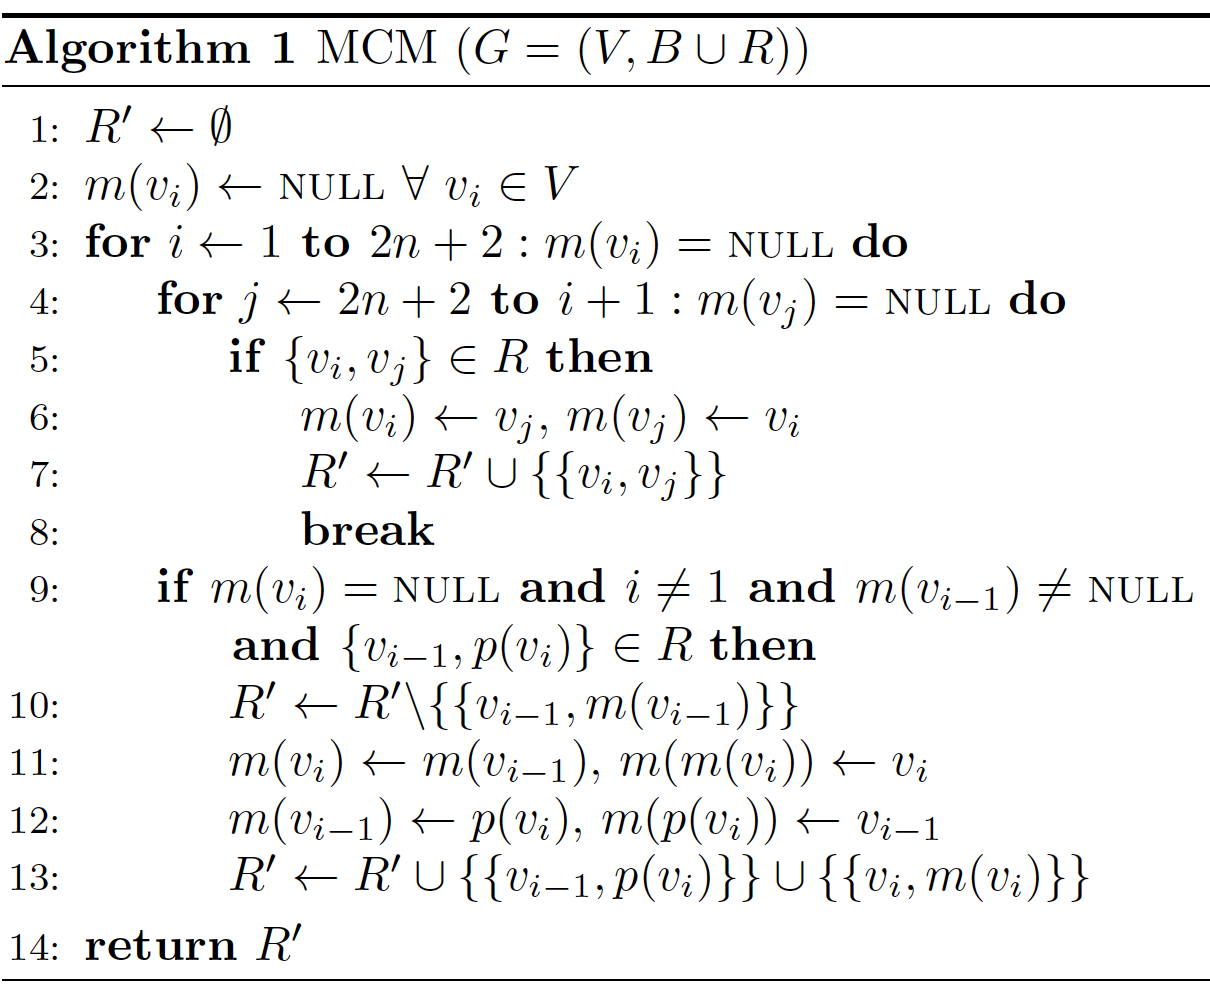
\includegraphics[width=0.48\textwidth]{figures/AlgMCMcrop1}
	\caption{Pseudocode for the Maximum Cardinality Matching (MCM) algorithm used within AHC to obtaining a matching $R'$ from the edge set $R$. Here, the \emph{match} of a vertex $v_i$ is denoted as $m(v_i)$.}	
	\label{fig:algmcm}
\end{figure}
\end{comment}

As shown in the pseudocode in Algorithm~\ref{alg:mcm}, vertices are considered in turn in weight-ascending order and are matched with the highest-weighted unmatched vertex adjacent in $R$. Here, the \emph{match} of a vertex $v_i$ is denoted as $m(v_i)$. The set $R'$ then consists of all edges from $R$ between matched vertices, i.e. $\{\{v_i, m(v_i)\} : v_i \in V \}$. In the event that a vertex $v_i$ is not adjacent to any other vertex via an edge in $R$, the previous vertex $v_{i-1}$ can be rematched provided $v_{i-1}$ has been matched successfully and is adjacent to $v_i$'s partner, $p(v_i)$. Then, $v_i$ is matched with $v_{i-1}$'s match, and $v_{i-1}$ is rematched with $p(v_i)$ (lines 9--13).

At this point, if $R'$ does not contain $n+1$ edges then there are too few edges to form an alternating Hamiltonian cycle, thus no feasible solution can exist and computation terminates. Otherwise, the spanning subgraph $G'=(V, B \cup R')$ will be a 2-regular graph consisting of cyclic components $C_1,C_2,\dotsc,C_z$ (as illustrated in Figs.~\ref{fig:matching} and~\ref{fig:mps}). Clearly, if $z = 1$, then $G'$ is an alternating Hamiltonian cycle and a solution has been found; otherwise $G'$ comprises multiple cycles, so AHC must find a way of connecting these components to form a single alternating Hamiltonian cycle.

\begin{figure}[h!]	
	\centering
	\begin{subfigure}[h]{0.33\textwidth}
		\includestandalone[width=\textwidth]{figures/threshold}
		\vspace{-2mm}
		\caption{$G = (V, B \cup R)$}
		\label{fig:threshold}
	\end{subfigure} \hspace{5mm}
	\begin{subfigure}[h]{0.33\textwidth}
		\includestandalone[width=\textwidth]{figures/matching}
		\vspace{-2mm}
		\caption{$G' = (V, B \cup R')$}
		\label{fig:matching}
	\end{subfigure} \hspace{7mm}
	\begin{subfigure}[h]{0.2\textwidth}
		\includestandalone[width=\textwidth]{figures/mps}
		\caption{$G' = (V, B \cup R')$}
		\label{fig:mps}
	\end{subfigure}
	\caption{(a) Graph $G$ modelling an example instance $\mathcal{M}$; (b) The subgraph $G'$ with $R' \subseteq R$ formed by MCM; (c) A planar embedding of $G'$ showing $z = 4$ components. Here, members of $B$ are shown by thick blue edges and $R$ by thin red edges, with vertex weights in parentheses.}
	\label{fig:mcm}
\end{figure}

To merge the components together, edges in $R'$ need to be replaced with new edges from $R \backslash R'$ that connect vertices from different components. The task involves deciding which particular edges to remove from $R'$, and which edges from $R \backslash R'$ to add to $R'$.

\subsubsection{Modifying the matching $R' \subseteq R$}
\label{subsub:bcr}
\noindent The second subprocedure of AHC is the Bridge-Cover Recognition (BCR) algorithm, based on a method by \cite{becker2010}. BCR seeks to identify subsets of edges in different components of $G'$ that will be removed from $R'$. These edge subsets are also used to identify the new edges from $R \backslash R'$ to be added to $R'$ that will then act as bridges, connecting those components into a single component. BCR aims to produce a collection $\mathcal{R}''$ of these subsets. Here, $\mathcal{R}''$ is said to \emph{cover} a component $C_j$ of $G'$ if there exists a subset in $\mathcal{R}''$ that contains an edge in $C_j$.

To begin, the edges in $R'$ are sorted into a list $\mathcal{L}$ such that the lower-weighted vertices of the edges are in ascending order (see Fig.~\ref{fig:bcrlist}). Then, in each iteration, BCR searches from the beginning of $\mathcal{L}$ to find two or more successive edges that meet the following conditions:
\begin{enumerate}[label={(\roman*)},itemsep=-0.2em]
	\item the lower-weighted vertex of each edge is adjacent to the higher-weighted vertex of the next edge via an edge in $R\backslash R'$;\label{item:adj}
	\item each edge is in a different component of $G'$; \label{item:diffcomp} and
	\item only one edge is in a component already covered by $\mathcal{R}''$; all other edges are in components not yet covered by $\mathcal{R}''$.\label{item:overlap}
\end{enumerate} 
These edges form a subset $R''_i$, which BCR adds to $\mathcal{R}''$ before continuing the search for another subset of edges.\footnote{When searching for edges to produce the first subset, $R''_1$, only Conditions \ref{item:adj} and \ref{item:diffcomp} are required since $\mathcal{R}'' = \emptyset$.} Once the penultimate edge in $\mathcal{L}$ has been assessed, edges in $\mathcal{R}''$ are removed from $\mathcal{L}$ and the next iteration begins. BCR ends the search successfully once $\mathcal{R}''$ covers all $z$ components of $G'$. However, if no new subsets are created during an iteration or if fewer than two edges remain in $\mathcal{L}$ after an iteration and $\mathcal{R}''$ does not cover all $z$ components, then no more subsets exist and it can be concluded with certainty that no feasible solution exists for the given instance of the COP. Fig.~\ref{fig:bcr} shows the BCR process on our example instance, where the subsets $R''_1 = \{\{v_2, v_{17}\},\{v_3, v_{16}\}, \{v_4, v_{15}\}\}$ and $R''_2 = \{\{v_7, v_{12}\}, \{v_8, v_{11}\}\}$ have been formed. As $\mathcal{R}'' =\{R''_1, R''_2\}$ covers all four components of $G'$, no more subsets are required.

Once a feasible collection $\mathcal{R}''$ has been produced, BCR uses each subset $R''_i \subset \mathcal{R}''$ to procure the replacement edges from $R\backslash R'$ as follows: for each edge in $R''_i$ in turn, the edge from $R \backslash R'$ connecting the lower-weighted vertex of the edge to the higher-weighted vertex of the next edge is added to $R'$. These edges form bridges between vertices of different components (as shown in Fig.~\ref{fig:mpsconnect}). The edges in $\mathcal{R}''$ are then removed from $R'$, so that $R'$ remains a perfect matching of cardinality $n+1$. This modified matching $R'$ along with the edge set $B$ will form an alternating Hamiltonian cycle in $G'$. Finally, removing the universal vertices yields an alternating Hamiltonian path which corresponds to a feasible solution $\mathcal{T}$ (Fig.~\ref{fig:solutionpath}).

\begin{figure}[h]	
	\centering
	\begin{subfigure}[h]{0.35\textwidth}
		\includestandalone[width=\textwidth]{figures/bcr}
		\caption{}
		\label{fig:bcrlist}
	\end{subfigure} \hspace{7mm} %
	\begin{subfigure}[h]{0.25\textwidth}
		\includestandalone[width=\textwidth]{figures/mpsconnect}
		\caption{}
		\label{fig:mpsconnect}
	\end{subfigure} \hspace{7mm} %
	\begin{subfigure}[h]{0.25\textwidth}
		\includestandalone[width=\textwidth]{figures/mpscycle}
		\caption{}
		\label{fig:mpscycle}
	\end{subfigure}
	\begin{subfigure}[h]{0.75\textwidth}
		\includestandalone[width=\textwidth]{figures/solutionpath}
		\caption{}
		\label{fig:solutionpath}
	\end{subfigure}
	\caption{BCR creates a collection $\mathcal{R}'' = \{R''_1, R''_2\}$ of subsets containing edges in $R'$ that when replaced by edges from $R\backslash R'$ connects the components of $G'$ into a single alternating Hamiltonian cycle. Dashed green edges and dotted orange edges are the bridges from $R''_1$ and $R''_2$ respectively. The resulting alternating Hamiltonian path corresponds to a solution $\mathcal{T}$.}
	\label{fig:bcr}
\end{figure}

\noindent In the first incarnation of this algorithm \citep{becker2010}, a procedure was used that searches through $\mathcal{L}$ just once to find edge subsets for the collection $\mathcal{R}''$. However, for some instances, although $\mathcal{R}''$ covers all components of $G'$ the components cannot be connected into a single alternating Hamiltonian cycle. This issue stems from the requirements for edges to form a subset, where originally Condition~\ref{item:overlap} allowed edges to be in multiple components already covered by $\mathcal{R}''$. This causes extra edges from $R \backslash R'$ to be added between components that have already been connected, resulting in multiple components being formed. Restricting Condition~\ref{item:overlap} such that only \emph{one} edge can be in a component covered by $\mathcal{R}''$ prevents these unnecessary additional edges from being included in $R'$, ensuring the components are linked to produce a single cycle. Fig.~\ref{fig:overlaperror} shows the formation of $\mathcal{R}''$ using the original procedure, where the subset $R''_2$ contains edges in \emph{two} components that $\mathcal{R}''$ already covers. Although $\mathcal{R}'' = \{R''_1, R''_2\}$ covers all components of $G'$, the bridges obtained from these subsets link $C_2$ and $C_3$ twice, thus connecting the four components into two different components. A further procedure was implemented by \cite{hawa2018} that recitifies this issue, but we found that the combination of both procedures was unnecessary. Therefore, we replace the two procedures with a single algorithm, BCR, that produces the same results in a more efficient manner.

\begin{figure}[h!]
	\centering	
	\begin{subfigure}[h]{0.35\textwidth}
		\includestandalone[width=\textwidth]{figures/bcrerror}
		\caption{}
		\label{fig:bcrerror}
	\end{subfigure} \hspace{5mm}
	\begin{subfigure}[h]{0.25\textwidth}
		\includestandalone[width=\textwidth]{figures/mpsconnecterror}
		\caption{}
		\label{fig:mpsconnecterror}
	\end{subfigure} \hspace{5mm}
	\begin{subfigure}[h]{0.25\textwidth}
		\includestandalone[width=\textwidth]{figures/mpscycleerror}
		\caption{}
		\label{fig:mpscycleerror}
	\end{subfigure}
	\caption{The procedure proposed by \cite{becker2010} creates subsets in $\mathcal{R}''$ each containing edges in both $C_2$ and $C_3$, resulting in two cyclic components in $G'$ as opposed to a single alternating Hamiltonian cycle.}	
	\label{fig:overlaperror}
\end{figure}

\begin{theorem}
	Let $G=(V, B \cup R)$ be a graph modelled from an instance $\mathcal{M}$ of cardinality $n$ of the COP. Then, AHC terminates in at most $O(n^2)$ time.
	\label{thm:ahc}
\end{theorem}

\begin{proof}
	The first subprocedure, MCM, produces an initial matching $R' \subseteq R$ in at most $O(n^2)$ time. Sorting the $n+1$ edges of $R'$ into a list $\mathcal{L}$ for the second subprocedure, BCR, requires $O(n\lg n)$ time. As $G'$ comprises a maximum of $\floor*{\frac{n+1}{2}}$ components and each subset $R''_i$ created in BCR must contain at least two edges from $R'$, it follows that the number of subsets in $\mathcal{R}''$ required to cover all components of $G'$ is bounded by $\floor*{\frac{n+1}{2}}-1$. At least one new subset $R''_i$ is created in each iteration of BCR, and removing edges from $\mathcal{L}$ can be performed in constant time, meaning that the task of producing the collection of subsets $\mathcal{R}''$ is of quadratic complexity $O(n^2)$. Up to $n+1$ edges in $R'$ may be replaced with edges from $R \backslash R'$, which can be executed in $O(n)$ time. Consequently, AHC has an overall worst case complexity of $O(n^2)$. 
\end{proof}	

%--------------------------------------------------------------------------------------
\section{Heuristics for the SCPP}
\label{sec:heur}
\noindent In this section we now consider the multi-bin version of the SubSCP, the Score-Constrained Packing Problem (SCPP), in which a set $\mathcal{I}$ of $n$ items are to be partitioned into a set of bins $\mathcal{S} = \{S_1, S_2,\dotsc,S_k\}$ according to Constraints~\eqref{eqn:allpacked}--\eqref{eqn:feasible}. Recall here that a bin $S_j \in \mathcal{F}$ if and only if the total width of items in the bin, $A(S_j) = \sum_{i \in S_j} w_i$ does not exceed the bin's capacity $W$, and the vicinal sum constraint \eqref{eqn:vsc} is fulfilled. An optimal solution for the SCPP is a solution comprising the fewest number of bins required to feasibly pack all items in $\mathcal{I}$. Therefore, the aim is to minimise the number of bins $k$.

The BPP is known to be NP-hard \citep{garey1979}, and since the SCPP generalises the BPP it follows that the SCPP is also NP-hard. Assuming $P \neq NP$, we therefore cannot hope to find an optimal solution for all instances of the SCPP in polynomial time. A well-known heuristic for the BPP is First-Fit (FF), a greedy algorithm that packs each item one by one in some given order into the lowest-indexed bin such that the capacity of the bin is not exceeded. It is known that there always exists at least one ordering of the items such that FF produces an optimal solution, though identifying such an ordering is itself NP-hard \citep{lewis2009}. An improvement on FF is the First-Fit Decreasing (FFD) heuristic, where items are considered in non-increasing order of size. It has been proven that the worst case for FFD is $\frac{11}{9}k + \frac{6}{9}$, and that this bound is tight \cite{dosa2007}. Similar heuristics include Best-Fit (BF), in which each item is packed into the fullest bin that can accommodate the item without being overfilled, and its offline counterpart Best-Fit Decreasing (BFD). A comprehensive overview of these heuristics and related methods can be seen in \cite{coffman1984}. More advanced heuristics for the BPP have been developed with positive results, such as the Minimum Bin Slack (MBS) heuristic \citep{gupta1999}, which focuses on packing each bin in turn rather than each item, and modifications of MBS such as the Perturbation-MBS' heuristic of \cite{fleszar2002}.

For the BPP, a basic lower bound for $k$ is the theoretical minimum, $t = \ceil*{\sum_{i=1}^{n} w_i / W}$ \citep{martello1990l}. Note, however, that $t$ will not perform as accurately for the SCPP as it fails to account for the vicinal sum constraint. For example, given a set of $n$ items in which the largest score width $b_i < \tau / 2$, it is clear that no pairs of score widths can fulfil the vicinal sum constraint and so each item must be packed into individual bins, thus $k = n$.

The vicinal sum constraint also introduces further differences in solutions for the BPP and SCPP. The obvious disparity is that of the ordering and orientation of the items in the bins: unimportant in the BPP, but vital for the feasibility of a solution for the SCPP. Another distinction arises when attempting to modify solutions. In the BPP, a bin remains feasible when an item is removed or a new item is added (provided the bin can accommodate the item), whereas for the SCPP this may render a bin infeasible as the new adjacent score widths may not abide by the vicinal sum constraint. Consequently, heuristics for the BPP will need to be adapted in order to produce feasible solutions for the SCPP.

As the SCPP is a relatively new problem, few methods have been seen in literature. Some basic heuristics were introduced by \cite{hawa2018}, two of which are based on the FFD heuristic for the BPP. The Modified First-Fit Decreasing (MFFD) heuristic performs in the same fashion as FFD with the additional step that an item $i$ can only be packed into a bin $S_j$ if the score width on the end of $S_j$ and one of $i$'s score widths, $a_i$ or $b_i$, meet the vicinal sum constraint. An advancement of this heuristic is MFFD$^+$, which incorporates the entire AHC algorithm. Rather than attempting to pack an item $i$ into the ends of a bin $S_j$, MFFD$^+$ calls upon AHC to find a feasible ordering of all items in $S_j$ \emph{and} item $i$, i.e. AHC is used to determine the membership of $\mathcal{F}$.\footnote{If an item $i$ is the first to be packed into a bin, it is placed in a regular orientation, $(a_i, b_i)$.} Clearly, MFFD$^+$ is the superior of the two, as the application of AHC guarantees that a feasible configuration of items in a bin will be found if it exists. To demonstrate this, Fig.~\ref{fig:mffdvsmffdplus} compares solutions produced using MFFD and MFFD$^+$ for the same instance of the SCPP. Note that MFFD$^+$ has formed an optimal solution, as it comprises $t = 6$ bins.

\begin{figure}[H]	
	\centering
	\begin{subfigure}[h]{0.33\textwidth}
		\includestandalone[width=\textwidth]{figures/mffd}
		\caption{MFFD}
		\label{fig:mffd}
	\end{subfigure} \hspace{15mm}
	\begin{subfigure}[h]{0.33\textwidth}
		\includestandalone[width=\textwidth]{figures/mffdplus}
		\caption{MFFD$^+$}
		\label{fig:mffdplus}
	\end{subfigure}
	\caption{Solutions formed using the MFFD and MFFD$^+$ heuristics. Here, $|\mathcal{I}| = 15$, $W = 1000$, and $\tau = 70$. As the theoretical minimum $t = 6$ bins, MFFD$^+$ has produced an optimal solution.}
	\label{fig:mffdvsmffdplus}
\end{figure}

%--------------------------------------------------------------------------------------
\section{An Evolutionary Algorithm for the SCPP}
\label{sec:ea}
\noindent We now introduce an evolutionary algorithm (EA) for the SCPP to improve on the heuristics discussed in the previous section. An evolutionary algorithm is a metaheuristic optimisation algorithm inspired by the natural evolutionary process. A set of candidate solutions to the problem form the initial population, and procedures emulating natural selection, reproduction, recombination and mutation are used to create the next generation of solutions. This iterated process results in the evolution of the population. Clearly, given large problem instances, the number of feasible packings will be too large to enumerate. However, we can incorporate the AHC algorithm for solving instances of the SubSCP into recombination operators within an EA, ensuring that feasible configuations will be found. EAs have been used for a variety of grouping problems with positive results \citep{lewis2017, falkenauer1996, quiroz2015}. Within the EA framework, we investigate three different group-based recombination operators as well as a local search procedure inspired by \cite{martello1990l}. The AHC algorithm described in Section~\ref{sec:ahc} is also integrated into the EA to solve instances of the SubSCP as and when they occur.

The most prominent reason for using evolutionary methods for the SCPP is because the number of packings can become too large to enumerate. In fact, in preliminary tests, we attempted to implement two sets, $\mathcal{X}$ and $\mathcal{Y}$, where $\mathcal{X}$ contained subsets $\mathcal{I}' \subset \mathcal{I}$ of items that were able to be packed feasibly into a single bin, and $\mathcal{Y}$ contained subsets of items that were unable to be packed feasibly into a single bin. As these sets were stored as binary trees, packings could be searched for and added to the sets in at most $O(\lg n)$ time. Thus, for any subset of items, AHC would only have to be executed at most once. However, during these preliminary tests, the size of $\mathcal{X}$ and $\mathcal{Y}$ became incredibly large such that the computers were unable to maintain the sets, resulting in the programs terminating prematurely and unsuccessfully. Furthermore, using an EA allows us to incorporate a variety of operators specifically designed for the SCPP, as well as a local search method which is able to move items \emph{between} bins, a useful property which the previous heuristics do not possess.

\subsection{Recombination}
\label{sub:recomb}
\noindent Recombination is used in EAs to generate new solutions by taking existing parent solutions and combining parts of them to create one or more offspring solutions. A recombination operator determines which elements from each parent should be inherited by the offspring. The operators implemented in our EA start with a single offspring $\mathcal{S} = \emptyset$, and uses two parent solutions, $\mathcal{S}_1$ and $\mathcal{S}_2$, to build the offspring solution. These operators are designed to ensure all bins in the offspring are feasible, though they can result in a partial offspring solution. In such cases, a repair procedure described below is used to re-establish a full solution $\mathcal{S}$.

The first operator is based on the grouping genetic algorithm (GGA) of \cite{falkenauer1992}. The bins of the second parent solution $\mathcal{S}_2$ are randomly permuted, and two bins $S_i$ and $S_j$ are selected randomly (where $1 \leq i < j \leq |\mathcal{S}_2|$). All bins between and including $S_i$ and $S_j$ are then copied into the offspring $\mathcal{S}$. Finally, GGA adds to the offspring all bins from $\mathcal{S}_1$ that do not contain any items already present in the offspring.

The second operator we implemented is the alternating grouping crossover (AGX), and is similar to that of \cite{quiroz2015} proposed for the BPP. Starting with the parent solution containing the fullest bin, AGX copies this bin into the offspring $\mathcal{S}$.\footnote{For both AGX and AGX', in the event that both parents contain bins with equal maximum fullness/number of items, the initial parent solution is chosen at random.} Then, bins containing any items in $\mathcal{S}$ are removed from both $\mathcal{S}_1$ and $\mathcal{S}_2$. The operator then proceeds by copying the fullest bin from the other parent solution into $\mathcal{S}$, and bins are removed from both parents as before. AGX continues to alternate between parents, selecting the fullest bin from each one until at most $\min (|\mathcal{S}_1|,|\mathcal{S}_2|) - 1$ bins have been added to the offspring solution.

Our final operator, AGX$'$, behaves in a similar manner to AGX; however rather than choosing the fullest bin to copy into the offspring, AGX$'$ selects bins containing the most items. Both AGX and AGX$'$ are based on the observation that in solutions with fewer bins, many of the bins will be well-filled. Thus, by selecting bins which are fuller or contain more items from parents to copy into the offspring $\mathcal{S}$, there is the potential to reduce the number of bins in $\mathcal{S}$ as fewer additional bins will be required to pack the remaining items during the repair procedure.

\begin{figure}[h!]	
	\centering
	\begin{minipage}{0.28\textwidth}
		\includestandalone[width=\textwidth]{figures/parentS1}
	\end{minipage} \hspace{15mm}
	\begin{minipage}{0.28\textwidth}
		\includestandalone[width=\textwidth]{figures/parentS2}
	\end{minipage}
\end{figure}

\begin{figure}[h!]	
	\centering
	\begin{subfigure}[h]{0.3\textwidth}
		\includestandalone[width=\textwidth]{figures/gga}
		\caption{GGA}
		\label{fig:gga}
	\end{subfigure} \hspace{5mm}
	\begin{subfigure}[h]{0.3\textwidth}
		\includestandalone[width=\textwidth]{figures/agx}
		\caption{AGX}
		\label{fig:agx}
	\end{subfigure} \hspace{5mm}
	\begin{subfigure}[h]{0.3\textwidth}
		\includestandalone[width=\textwidth]{figures/agxdash}
		\caption{AGX$'$}
		\label{fig:agxdash}
	\end{subfigure}
	\caption{Partial offspring solutions and missing items created from parent solutions $\mathcal{S}_1$ and $\mathcal{S}_2$ using our different recombination operators. In (a), GGA has copied bins $S_2, S_3$ and $S_4$ from $\mathcal{S}_2$ to the offspring, and in (b) and (c) $\mathcal{S}_1$ is the initial parent for both AGX and AGX$'$ as it contains both the fullest bin and the bin with the most items.}
	\label{fig:recomb}
\end{figure}

\noindent As explained in the previous section, removing an item from a bin in a solution for the SCPP may result in a violation of the vicinal sum constraint. Therefore, in order to maintain feasibility of each bin, the operators disregard entire bins in the parent solutions that contain items already in the offspring, rather than removing individual items. These excluded bins, however, may also hold items that are not yet present in the offspring $\mathcal{S}$. Consequently, on completion of the recombination, $\mathcal{S}$ will be a partial solution. To rectify this, the following repair procedure is implemented. Firstly,the MFFD$^+$ heuristic described in Section~\ref{sec:heur} is applied using just the missing items to form a second partial solution $\mathcal{S}'$. Then, both $\mathcal{S}$ and $\mathcal{S}'$ are used as input into a local search procedure, producing a full feasible offspring solution. Fig.~\ref{fig:recomb} shows the partial offspring $\mathcal{S}$ produced from two parent solutions using each of the recombination operators, along with the individual items missing from each offspring.

\subsection{Local Search}
\label{sub:localsearch}
\noindent As previously mentioned, our local search method takes two partial solutions $\mathcal{S}$ and $\mathcal{S}'$ containing bins that, together, form a full solution containing all items in $\mathcal{I}$. The aim of this local search is to strategically shuffle items between the bins of each partial solution. Specifically, we seek to increase the fullness $A(S_j)$ of bins $S_j \in \mathcal{S}$ while maintaining or decreasing the number of items in these bins. As a result, items moved into $\mathcal{S}'$ will be smaller and therefore easier to repack into bins in $\mathcal{S}$ later. The procedure begins by permuting the bins in $\mathcal{S}$ and $\mathcal{S}'$, before attempting to exchange items in four stages:
\begin{enumerate}[label={(\arabic*)},itemsep=-0.2em]
	\item swapping a pair of items from a bin in $\mathcal{S}$ with a pair of items from a bin in $\mathcal{S}'$;\label{item:pairpair}
	\item swapping a pair of items from a bin in $\mathcal{S}$ with an individual item from a bin in $\mathcal{S}'$;\label{item:pairsin}
	\item swapping individual items from bins in $\mathcal{S}$ and $\mathcal{S}'$;\label{item:sinsin} and
	\item moving an item from a bin in $\mathcal{S}'$ to a bin in $\mathcal{S}$.\label{item:movesin}
\end{enumerate} 
During Stages \ref{item:pairpair}--\ref{item:sinsin}, the width of the item(s) from $\mathcal{S}'$ must exceed the width of the item(s) from $\mathcal{S}$. In each stage, AHC is executed on the modified groups of items in each bin, and the items are permanently moved only if AHC finds feasible packings for both bins. Once an exchange occurs, the procedure immediately proceeds to the next stage. This process is repeated until all four stages have been conducted in succession with no changes to $\mathcal{S}$ or $\mathcal{S}'$. Next, MFFD$^+$ is applied to any items remaining in $\mathcal{S}'$, generating a new feasible partial solution $\mathcal{S}''$. Finally, the bins in $\mathcal{S}''$ are moved into $\mathcal{S}$, resulting in a full solution.

This method is based on the dominance criterion of \cite{martello1990l} for the BPP. Variations of this method can be seen in \cite{falkenauer1996}, \cite{levine2004}, \cite{lewis2009}, and \cite{lewis2017}; however the addition of the vicinal sum constraint will often result in fewer changes than seen in these previous implementations.

\subsection{Evolutionary Algorithm Framework}
\label{sub:eaframework}
\noindent Our EA for the SCPP begins by producing candidate solutions to form an initial population, with one solution created using MFFD$^+$ and the rest using MFFR$^+$ (where items are packed in random order). Each solution is mutated before being inserted into the population. The mutation of a solution $\mathcal{S}$ consists of permuting the bins, moving $1 < r < |\mathcal{S}|$ bins selected randomly from $\mathcal{S}$ into a set $\mathcal{S}'$, and then executing local search on these two partial solutions to produce a full feasible solution $\mathcal{S}$. Each iteration of the EA involves selecting two parent solutions, $\mathcal{S}_1$ and $\mathcal{S}_2$, from the population at random, applying a recombination operator to produce an offspring solution $\mathcal{S}$, then finally mutating $\mathcal{S}$ before replacing the least fit of the two parents in the population.

As with other BPP algorithms, we use the following function introduced by \cite{falkenauer1992} to calculate the fitness of a solution $\mathcal{S}$:
\begin{equation}
f(\mathcal{S}) = \frac{\sum_{S_j \in \mathcal{S}} (A(S_j)/W)^2}{|\mathcal{S}|}
\label{eqn:fitness}
\end{equation}

\noindent which assigns higher values to higher quality solutions. This is more fine-grained than simply using the number of bins, and provides greater distinction between solutions, therefore allowing evolutionary pressure to be maintained for longer periods during a run. For the BPP, it can be shown that if $|\mathcal{S}_1| < |\mathcal{S}_2|$  then $f(\mathcal{S}_1) > f(\mathcal{S}_2)$, hence a global optimum for this fitness function is associated with the optimal solution containing the fewest number of bins, provided that there exists at most one bin that is less than half full in each solution \citep{falkenauer1998}. This is true for the BPP when in conjunction with algorithms such as FF, but this is not always the case with the SCPP due to the vicinal sum constraint. We therefore use this fitness function as a secondary evaluation to identify the higher quality solution when faced with solutions comprising the same number of bins.

\subsection{Experimental Results - EA}
\label{sub:expea}
\noindent Our EA was executed on a set of problem instances for the SCPP created using a problem instance generator available online \citep{hawa2019inst}. The set contains two types of problem instances: ``artificial'', in which the items are strongly heterogeneous (the items have varying widths and score widths); and ``real'', where items are weakly hetergeneous (many items have the same dimensions). Each type contains three subsets of 1000 instances for 100, 500, and 1000 items, giving a total of 6000 problem instances. All items have widths $w_i \in [150,1000]$ and score widths $a_i, b_i \in [1,70]$ selected uniform randomly, and equal height $H=1$. For the real instances, the number of item types was chosen uniform randomly between 10 and 30, and the number of items within each group also assigned uniform randomly.

Two different bin sizes, $W = 2500$ and 5000 (also of height $H=1$), were used in the experiments in order to help alter the number of items per bin, and the minimum scoring distance $\tau$ was set to 70mm -- the industry standard. After preliminary experiments, we settled for an initial population containing 25 candidate solutions. Across all instances, the EA was granted a fixed time limit of 600 seconds. The MFFD$^+$ heuristic descibed in Section~\ref{sec:heur} was also executed on the same set of problem instances to provide comparative results. Table~\ref{table:ea} displays the results obtained from the experiments using the different recombination operators and bin sizes, which can be found online along with all of our source code \citep{hawa2019ea}.\footnote{All experiments were implemented in C++ and executed on Windows machines with Intel Core i5-6500 3.20GHz processors and 8GB of RAM.}

\begin{table}[h]
%\setlength{\tabcolsep}{3pt}
\centering
\caption{Best solutions obtained from the EA using the GGA, AGX, and AGX$'$ recombination operators, and from the MFFD$^+$ heuristic. Figures in bold indicate the best results for each instance class. Asterisks indicate statistical significance at $\leq 0.05 (^{*})$ and $\leq 0.01 (^{**})$ according to a two-tailed paired t-test and two-tailed McNemar's test for the $|\mathcal{S}|$ and $\%t$ columns respectively. Note that the statistical tests were only performed on the recombination operators.}
%\tiny
\begin{threeparttable}
\resizebox{\textwidth}{!}{%
\begin{tabular}{crrcrrcrrcrrcrr}
	\toprule
	& & & & \multicolumn{2}{c}{GGA} &\phantom{}& \multicolumn{2}{c}{AGX} &\phantom{}& \multicolumn{2}{c}{AGX$'$} &\phantom{} & \multicolumn{2}{c}{MFFD$^+$}\\
	\cmidrule{5-6} \cmidrule{8-9} \cmidrule{11-12} \cmidrule{14-15}
	\multicolumn{1}{c}{Type, $W$} & \multicolumn{1}{c}{$|\mathcal{I}|$} & \multicolumn{1}{c}{$t$\tnote{$a$}} && \multicolumn{1}{c}{$|\mathcal{S}|$\tnote{$b$}} & \multicolumn{1}{c}{$\% t$\tnote{$c$}} && \multicolumn{1}{c}{$|\mathcal{S}|$} & \multicolumn{1}{c}{$\% t$} && \multicolumn{1}{c}{$|\mathcal{S}|$} & \multicolumn{1}{c}{$\% t$} && \multicolumn{1}{c}{$|\mathcal{S}|$} & \multicolumn{1}{c}{$\% t$}\\
	\midrule
	a, 2500 & 100 & 23.32 && $23.36 \pm 4.6$ & 97.4 && $^{**}\textbf{23.34} \pm 4.5$ & $^{**}\textbf{98.6}$ && $23.36 \pm 4.5$ & 97.2 && $28.46 \pm 10.4$ & 2.6 \\
	& 500 & 114.94 && $116.36 \pm 2.2$ & 33.4 && $116.67 \pm 2.2$ & 27.4 && $^{**}\textbf{116.28} \pm 2.2$ &\textbf{35.0} && $132.65 \pm 4.9$ & 0.0 \\
	& 1000 & 229.44 && $233.93 \pm 1.6$ & 1.5 && $234.58 \pm 1.6$ & 1.3 && $^{**}\textbf{233.73} \pm 1.6$ &\textbf{2.3} && $258.39 \pm 3.5$ & 0.0 \\
	\midrule
	a, 5000 & 100 & 11.92 && $^{**}\textbf{12.27} \pm 10.0$ & $^{**}\textbf{84.5}$ && $12.31 \pm 10.2$ & 82.7 && $12.32 \pm 10.2$ & 82.0 && $19.88 \pm 18.3$ & 0.7 \\
	& 500 & 57.72 && $^{**}\textbf{61.91} \pm 4.9$ & \textbf{6.0} && $62.44 \pm 5.1$ & 4.5 && $62.50 \pm 5.0$ & 4.9 && $89.54 \pm 9.3$ & 0.0 \\
	& 1000 & 114.97 && $^{**}\textbf{126.37} \pm 4.0$ & 0.0 && $126.85 \pm 3.9$ & 0.0 && $127.08 \pm 4.0$ & 0.0 && $172.61 \pm 7.1$ & 0.0 \\
	\midrule
	\midrule
	r, 2500 & 100 & 23.47 && $25.99 \pm 21.3$ & \textbf{57.3} && $26.07 \pm 21.5$ & 57.0 && $^{*}\textbf{25.95} \pm 21.1$ & 57.0 && $35.42 \pm 23.1$ & 1.6 \\
	& 500 & 115.24 && $\textbf{133.94} \pm 21.3$ & 4.7 && $134.25 \pm 21.5$ & \textbf{5.9} && $133.99 \pm 21.2$ & 4.1 && $177.25 \pm 21.2$ & 0.0 \\
	& 1000 & 229.95 && $\textbf{269.99} \pm 21.6$ & 0.1 && $270.17 \pm 21.7$ & \textbf{0.4} && $270.03 \pm 21.6$ & 0.1 && $355.04 \pm 21.2$ & 0.0 \\
	\midrule
	r, 5000 & 100 & 11.98 && $\textbf{17.51} \pm 47.5$ & $^{*}\textbf{48.0}$ && $17.54 \pm 47.3$ & 46.8 && $17.54 \pm 47.2$ & 46.2 && $29.61 \pm 32.7$ & 0.5 \\
	& 500 & 57.87 && $^{**}\textbf{93.59} \pm 43.0$ & \textbf{8.7} && $94.18 \pm 43.0$ & 8.6 && $93.97 \pm 42.9$ & 8.0 && $153.42 \pm 28.9$ & 0.0 \\
	& 1000 & 115.23 && $^{**}\textbf{192.38} \pm 42.7$ & \textbf{3.1} && $192.92 \pm 42.8$ & 2.6 && $192.79 \pm 42.7$ & 3.0 && $308.64 \pm 28.7$ & 0.0 \\
	\bottomrule
\end{tabular}}	
\vspace{0.2cm} %
\begin{tablenotes}
	\tiny
	\item[$a$] $t = \ceil{\sum_{i=1}^{n} w_i / W}$ (mean from 1000 instances).
	\item[$b$] Number of bins per solution (mean from 1000 instances plus or minus the coefficient of variation (\%)).
	\item[$c$] Percentage of instances in which the solution comprises $t$ bins.
\end{tablenotes}
\end{threeparttable}
\label{table:ea}
\end{table}

It is immediately evident that all EA versions outperform the MFFD$^+$ heuristic, with superior averages in all cases. As $|\mathcal{I}|$ and $W$ are increased, fewer iterations of the EA are performed as the rise in both the number of bins in solutions and the number of items per bin results in many more applications of AHC within the local search procedure, thus taking longer for it to complete. For example, the average number of iterations ranged from 360,000 to 1200 when $W=2500$ for artificial instances using 100 and 1000 items respectively, whilst the corresponding figures for real instances using $W=5000$ were 55,000 and 65 iterations. Consequently, we see that the difference between $|\mathcal{S}|$ and the theoretical minimum $t$ also increases as the number of items increases, more so for the larger bin size. The reduction in the number of EA iterations means that the evolution of the population is restricted which prevents better solutions from being achieved, suggesting that the algorithm is less accurate.

\noindent We also observe that the coefficient of variation is considerably higher for real instances than for artificial instances. It is clear that $t$ will be less accurate for real instances due to the lack of item diversity and so, unlike with artificial instances, for each individual real problem instance the number of bins in the final solution may differ drastically from one another, resulting in a higher coefficient of variation.

The different recombination operators seem to perform well with different types of problem instance. GGA consistently produces the best results for both artificial and real instances using the larger bin size, where high quality solutions contain approximately 8.6 items per bin on average. The lack of bias in choice of bins to inherit allows more of the solution space to be explored, resulting in better solutions being found. AGX$'$ also appears to perform well when $W=2500$, where the best solutions average 4.3 items per bin. With regards to the average number of bins $|\mathcal{S}|$, AGX$'$ produces the best solutions for three of the six instance classes using the smaller bin size. For the remaining three classes, the result from AGX$'$ uses at most 0.05 bins more than the best result found. By selecting bins containing the most items, AGX$'$ aims to build solutions comprising fewer yet fuller bins, thus AGX$'$ is focused on higher quality individual bins as opposed to entire solutions.

AGX generates the least favourable results, particularly for real instances, where it is outperformed by GGA and AGX$'$ in all six instance classes with regards to the average number of bins per solution $|\mathcal{S}|$. Selecting bins based on fullness may mean choosing bins containing fewer items, thus requiring extra bins to pack all items. However, note that AGX yields the highest number of solutions comprising $t$ bins in three of the instance classes, suggesting a high variance in the quality of solutions produced.

%--------------------------------------------------------------------------------------
\section{A Hybrid Metaheuristic Approach to the SCPP}
\label{sec:cmsa}
\noindent In this section, we now explore an alternative approach to the SCPP that uses a hybrid metaheuristic method based on exact covering. To begin, we introduce the following definition:

\begin{definition}
	Let $\mathcal{B}$ be a collection of subsets of a set $\mathcal{I}$. Then, a subcollection $\mathcal{S}^*$ of $\mathcal{B}$ is an \emph{exact cover} if and only if each element in $\mathcal{I}$ is contained in exactly one subset in $\mathcal{S}^*$.
	\label{defn:exactcover}
\end{definition}	

\noindent For example, given a collection of subsets $\mathcal{B} = \{\{1,2,3\}, \{3,4,5\}, \{4\}, \{5\}\}$ of a set $\mathcal{I} = \{1,2,3,4,5\}$, the subcollection $\mathcal{S}^*_1 = \{\{1,2,3\}, \{3,4,5\}\}$ is a set cover as it contains every element of $\mathcal{I}$, whereas the subcollection $\mathcal{S}^*_2 = \{\{1,2,3\}, \{4\}, \{5\}\}$ is an \emph{exact cover} as it contains every element of $\mathcal{I}$ exactly once. The exact cover problem, determining whether a exact cover $\mathcal{S}^*$ of $\mathcal{B}$ exists, is a decision problem and one of the original 21 NP-complete problems \citep{karp1972}. If it is known that an exact cover exists, the problem can also be reformulated as an NP-hard optimisation problem with the objective of finding the smallest subcollection.

Given a set of feasible bins $\mathcal{B}$ for an instance of the SCPP, it can be seen that finding a solution $\mathcal{S}^*$ is in fact an exact cover problem. Since the bins are already feasible, the complications associated with the vicinal sum constraint are eliminated.

Ideally, every element in the set of feasible bins $\mathcal{F}$ would correspond to a member of $\mathcal{B}$, however since the cardinality of $\mathcal{F}$ has the potential to grow at an exponential rate in relation to the problem size it may not be possible to produce $\mathcal{B}$ in this manner, let alone find an exact cover in a feasible amount of time. One option is to implement a method of finding an exact cover within the Construct, Merge, Solve \& Adapt (CMSA) algorithm of \cite{blum2016}. Rather than having a population of full solutions as used in our EA, CMSA operates on the set $\mathcal{B}$ of individual feasible bins.
\begin{comment}
\begin{figure}[h!]	
	\centering
	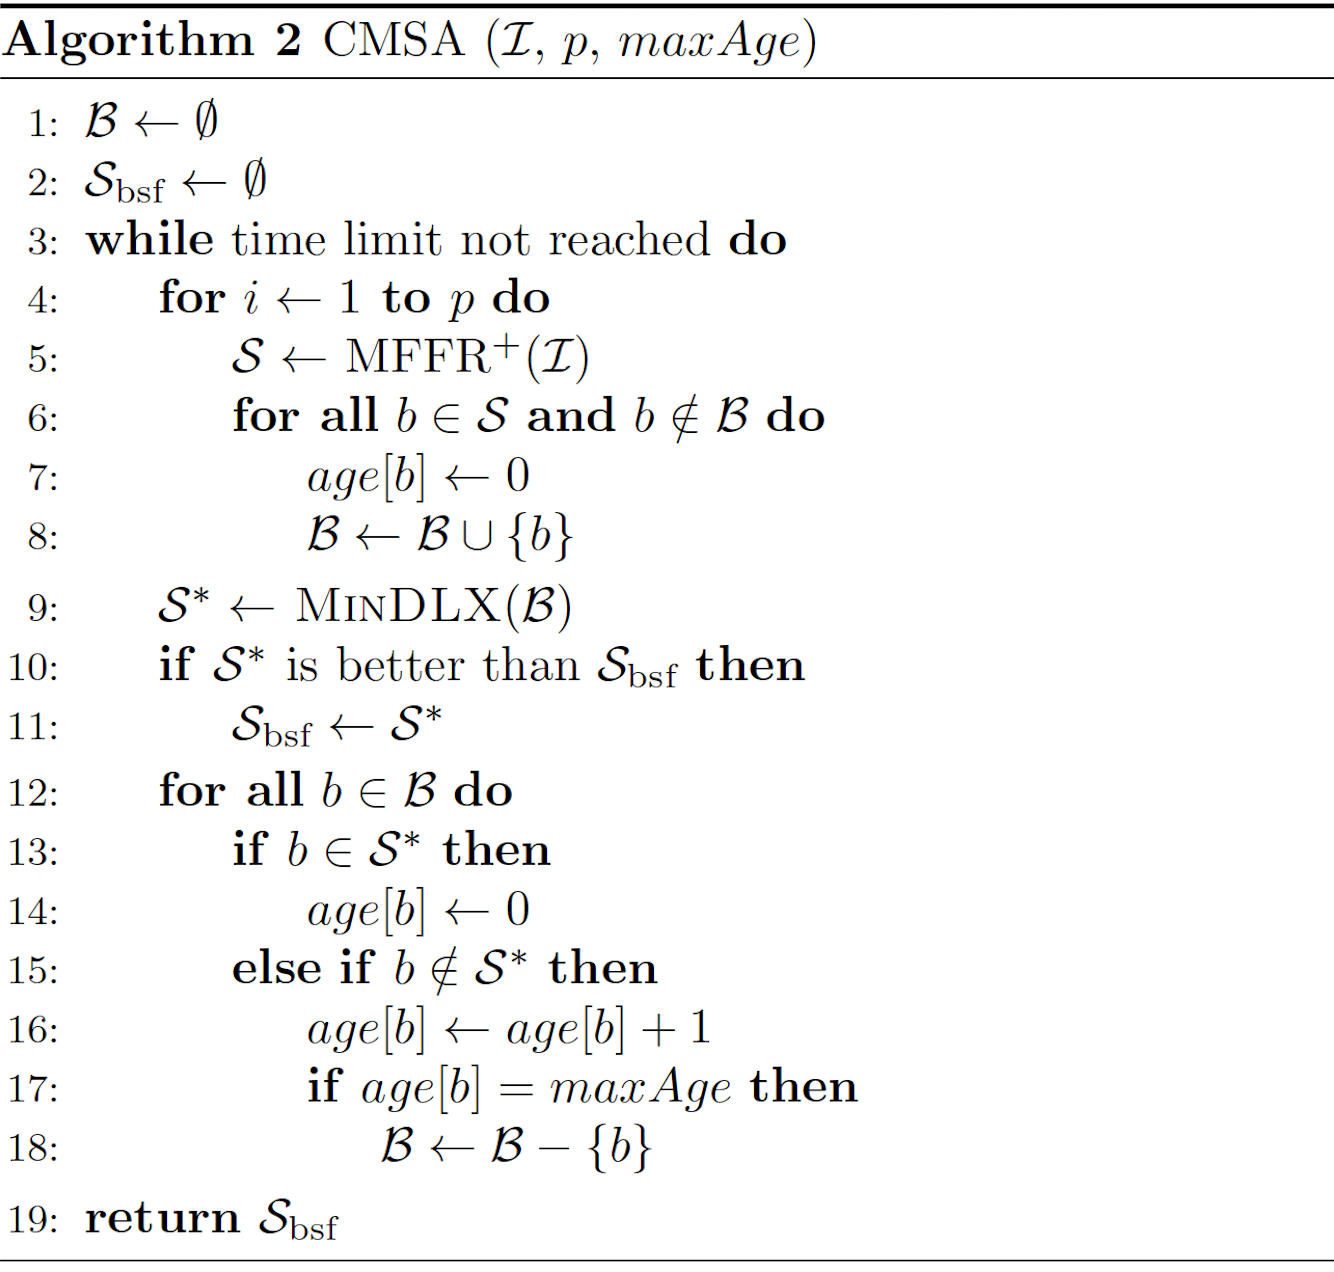
\includegraphics[width=0.48\textwidth]{figures/AlgCMSAcrop3}
	\caption{Pseudocode for the Construct, Merge, Solve \& Adapt (CMSA) algorithm for the SCPP, which uses our \textsc{MinDLX} algorithm to find a minimum cardinality exact cover.}	
	\label{fig:algcmsa}
\end{figure}
\end{comment}

The pseudocode for CMSA is provided in Algorithm~\ref{alg:cmsa}. Firstly, a fixed number $p$ of solutions are produced using MFFR$^+$. The bins of each solution are inserted into the set $\mathcal{B}$, and the age of every bin is set to zero (lines 4--8). CMSA then calls upon the \textsc{MinDLX} algorithm (described below) to find a minimum cardinality exact cover $\mathcal{S}^*$ of set $\mathcal{B}$, which, if better than the best-so-far solution $\mathcal{S}_{\textup{bsf}}$, is stored as the new best-so-far solution (lines 9--11). The set $\mathcal{B}$ is then adapted by resetting the age of bins used in $\mathcal{S}^*$ to zero and increasing the age of all other bins by one (lines 12--16). Finally, any bins in $\mathcal{B}$ whose age has reached the maximum are removed from the set (lines 17--18). This process is repeated until a set time limit has been reached. The adaptation stage aids the process by removing bins from $\mathcal{B}$ that have not contributed to an optimal solution for a set period of time. This allows the algorithm to control the size of $\mathcal{B}$ and thus the speed of the exact solver. It also retains bins in $\mathcal{B}$ that are used in solutions, which could prove to be useful in subsequent iterations of CMSA.

\begin{algorithm}[h!]
\caption{CMSA ($\mathcal{I}$, $p$, $maxAge$)}
\begin{algorithmic}[1]
	\State $\mathcal{B} \gets \emptyset$
	\State $\mathcal{S}_{\textup{bsf}} \gets \emptyset$
	\While{time limit not reached}
		\For{$i\gets 1 \To p$}
			\State $\mathcal{S} \gets$ MFFR$^+$($\mathcal{I}$)
			\ForAll{$b \in \mathcal{S}$ \textbf{and} $b \notin \mathcal{B}$}
				\State $age[b] \gets 0$
				\State $\mathcal{B} \gets \mathcal{B} \cup \{b\}$
			\EndFor
		\EndFor
		\State $\mathcal{S}^* \gets$ \textsc{MinDLX}($\mathcal{B}$)
		\If{$\mathcal{S}^*$ is better than $\mathcal{S}_{\textup{bsf}}$}
			\State $\mathcal{S}_{\textup{bsf}} \gets \mathcal{S}^*$
		\EndIf
		\ForAll{$b \in \mathcal{B}$}
			\If{$b \in \mathcal{S}^*$}
				\State $age[b] \gets 0$
			\ElsIf{$b \notin \mathcal{S}^*$}
				\State $age[b] \gets age[b] + 1$
				\If{$age[b] = maxAge$}
					\State $\mathcal{B} \gets \mathcal{B} - \{b\}$
				\EndIf
			\EndIf		
		\EndFor
	\EndWhile
	\Return $\mathcal{S}_{\textup{bsf}}$
\end{algorithmic}
\label{alg:cmsa}	
\end{algorithm}	

To find an exact cover, we use a recursive depth-first backtracking process implemented using the ``dancing links'' technique of \cite{knuth2000}. In general this algorithm, known as DLX, is designed to find all exact covers to a given problem instance. As we are only interested in determining a single minimum cardinality exact cover (i.e. a solution with the fewest bins) we modified this algorithm to create \textsc{MinDLX}, which only searches for solutions that improve upon the best solution found so far.

\subsection{Experimental Results - CMSA}
\label{sub:expcmsa}
\noindent Table~\ref{table:cmsa} compares the performance of the CMSA and EA algorithms on 50 randomly selected instances from each of the 12 instance classes. A time limit of 3600 seconds was used for the overall CMSA algorithm, while \textsc{MinDLX} was set to run for a maximum of 600 seconds in each iteration, which was deemed necessary in our initial trials. Parameter settings of $p = 3$ and $maxAge = 3$ were also decided after preliminary tests. For a fair comparison, we also ran our EA on the 50 instances for 3600 seconds each, to compare the three recombination operators in the EA with CMSA. The source code for the CMSA algorithm including the modified \textsc{MinDLX} procedure is also available online \citep{hawa2019cmsa}.

\begin{comment}
\begin{table}[h]
%\setlength{\tabcolsep}{3pt}
\centering
\caption{Results obtained from the CMSA algorithm and the EA using the three recombination operators. Figures in bold and asterisks should be interpreted as in Table~\ref{table:ea}.}
%\scriptsize
\begin{threeparttable}
\resizebox{\textwidth}{!}{%
\begin{tabular}{crrcrrcrrcrrcrr}
	\toprule
	& & & & \multicolumn{2}{c}{CMSA} &\phantom{}& \multicolumn{2}{c}{GGA} &\phantom{}& \multicolumn{2}{c}{AGX} &\phantom{} & \multicolumn{2}{c}{AGX$'$}\\
	\cmidrule{5-6} \cmidrule{8-9} \cmidrule{11-12} \cmidrule{14-15}
	\multicolumn{1}{c}{Type, $W$} & \multicolumn{1}{c}{$|\mathcal{I}|$} & \multicolumn{1}{c}{$t$\tnote{$a$}} && \multicolumn{1}{c}{$|\mathcal{S}|$\tnote{$b$}} & \multicolumn{1}{c}{$\# t$\tnote{$c$}} && \multicolumn{1}{c}{$|\mathcal{S}|$} & \multicolumn{1}{c}{$\# t$} && \multicolumn{1}{c}{$|\mathcal{S}|$} & \multicolumn{1}{c}{$\# t$} && \multicolumn{1}{c}{$|\mathcal{S}|$} & \multicolumn{1}{c}{$\# t$}\\
	\midrule
	a, 2500 & 100 & 23.36 && $24.02 \pm 5.5$ & 21 && $23.38 \pm 4.6$ & 49 && $\textbf{23.36} \pm 4.5$ & \textbf{50} && $\textbf{23.36} \pm 4.5$ & \textbf{50} \\
	& 500 & 114.74 && $118.48 \pm 2.3$ & 0 && $115.72 \pm 1.9$ & \textbf{20} && $ 116.26 \pm 1.9$ & 15 && $\textbf{115.64} \pm 1.9$ & \textbf{20} \\
	& 1000 & 230.24 && $237.10 \pm 1.8$ & 0 && $233.98 \pm 1.8$ & \textbf{2} && $235.00 \pm 1.8$ & 0 && $\textbf{233.80} \pm 1.7$ & \textbf{2} \\
	\midrule
	a, 5000 & 100 & 11.96 && $13.54 \pm 17.4$ & 24 && $\textbf{12.50} \pm 11.3$ & \textbf{39} && $12.54 \pm 11.7$ & \textbf{39} && $12.54 \pm 11.5$ & \textbf{39} \\
	& 500 & 57.62 && $75.60 \pm 9.8$ & 0 && $^{*}\textbf{60.96} \pm 3.9$ & \textbf{4} && $61.38 \pm 3.9$ & 3 && $ 61.78 \pm 4.3$ & 0 \\
	& 1000 & 115.42 && $169.04 \pm 8.5$ & 0 && $^{**}\textbf{124.42} \pm 4.5$ & 0 && $125.50 \pm 4.3$ & 0 && $126.40 \pm 4.5$ & 0 \\
	\midrule
	\midrule
	r, 2500 & 100 & 23.34 && $27.94 \pm 27.5$ & 15 && $\textbf{27.28} \pm 28.4$ & 23 && $ 27.58 \pm 28.5$ & 23 && $27.32 \pm 28.4$ & \textbf{24} \\
	& 500 & 115.76 && $148.04 \pm 27.1$ & 0 && $\textbf{142.26} \pm 26.6$ & 4 && $142.90 \pm 26.5$ & \textbf{6} && $143.06 \pm 26.3$ & 2 \\
	& 1000 & 231.26 && $294.76 \pm 27.1$ & 0 && $\textbf{289.16} \pm 26.1$ & 0 && $290.28 \pm 26.2$ & 0 && $290.36 \pm 26.2$ & 0 \\
	\midrule
	r, 5000 & 100 & 11.94 && $20.94 \pm 52.0$ & 12 && $\textbf{20.28} \pm 53.4$ & \textbf{17} && $20.38 \pm 53.0$ & 15 && $20.46 \pm 52.6$ & 15 \\
	& 500 & 58.12 && $113.96 \pm 46.5$ & 6 && $\textbf{107.66} \pm 47.1$ & \textbf{7} && $108.80 \pm 46.7$ & 5 && $108.24 \pm 46.4$ & 4 \\		
	& 1000 & 115.92 && $239.28 \pm 43.9$ & 0 && $\textbf{222.26} \pm 45.8$ & 0 && $223.44 \pm 45.6$ & 0 && $223.36 \pm 45.5$ & 0 \\
	\bottomrule
\end{tabular}}	
\vspace{0.2cm} %
\begin{tablenotes}
	\tiny
	\item[$a$] $t = \ceil{\sum_{i=1}^{n} w_i / W}$ (mean from 50 instances).
	\item[$b$] Number of bins per solution (mean from 50 instances plus or minus the coefficient of variation (\%)).
	\item[$c$] Number of instances in which the solution comprises $t$ bins.
\end{tablenotes}
\end{threeparttable}
\label{table:cmsavsea}
\end{table}
\end{comment}

\begin{table}[h]
%\setlength{\tabcolsep}{3pt}
\centering
\caption{Results obtained from the CMSA algorithm and the EA using the three recombination operators. Figures in bold and asterisks should be interpreted as in Table~\ref{table:ea}.}
%\scriptsize
\begin{threeparttable}
\resizebox{\textwidth}{!}{%
\begin{tabular}{crr c rrr c rrr c rrr c rrr}
	\toprule
	& & & & \multicolumn{3}{c}{CMSA} &\phantom{}& \multicolumn{3}{c}{GGA} &\phantom{}& \multicolumn{3}{c}{AGX} &\phantom{} & \multicolumn{3}{c}{AGX$'$}\\
	\cmidrule{5-7} \cmidrule{9-11} \cmidrule{13-15} \cmidrule{17-19}
	\multicolumn{1}{c}{Type, $W$} & \multicolumn{1}{c}{$|\mathcal{I}|$} & \multicolumn{1}{c}{$t$\tnote{$a$}} && \multicolumn{1}{c}{$|\mathcal{S}|$\tnote{$b$}} & \multicolumn{1}{c}{$\# t$\tnote{$c$}} & \multicolumn{1}{r}{Best\tnote{$d$}}  && \multicolumn{1}{c}{$|\mathcal{S}|$} & \multicolumn{1}{c}{$\# t$} & \multicolumn{1}{r}{Best} && \multicolumn{1}{c}{$|\mathcal{S}|$} & \multicolumn{1}{c}{$\# t$} & \multicolumn{1}{r}{Best} && \multicolumn{1}{c}{$|\mathcal{S}|$} & \multicolumn{1}{c}{$\# t$} & \multicolumn{1}{r}{Best}\\
	\midrule
	a, 2500 & 100 & 23.36 && $24.02 \pm 5.5$ & 21 & 0 && $23.38 \pm 4.6$ & 49 & 0 && $\textbf{23.36} \pm 4.5$ & \textbf{50} & 0 && $\textbf{23.36} \pm 4.5$ & \textbf{50} & 0 \\
	& 500 & 114.74 && $118.48 \pm 2.3$ & 0 & 0 && $115.72 \pm 1.9$ & \textbf{20} & 5 && $ 116.26 \pm 1.9$ & 15 & 1 && $\textbf{115.64} \pm 1.9$ & \textbf{20} & \textbf{9} \\
	& 1000 & 230.24 && $237.10 \pm 1.8$ & 0 & 0 && $233.98 \pm 1.8$ & \textbf{2} & 10 && $235.00 \pm 1.8$ & 0 & 1 && $\textbf{233.80} \pm 1.7$ & \textbf{2} & \textbf{15} \\
	\midrule
	a, 5000 & 100 & 11.96 && $13.54 \pm 17.4$ & 24 & 0 && $\textbf{12.50} \pm 11.3$ & \textbf{39} & \textbf{2} && $12.54 \pm 11.7$ & \textbf{39} & 0 && $12.54 \pm 11.5$ & \textbf{39} & 0 \\
	& 500 & 57.62 && $75.60 \pm 9.8$ & 0 & 0 && $^{*}\textbf{60.96} \pm 3.9$ & \textbf{4} & \textbf{17} && $61.38 \pm 3.9$ & 3 & 6 && $ 61.78 \pm 4.3$ & 0 & 2 \\
	& 1000 & 115.42 && $169.04 \pm 8.5$ & 0 & 0 && $^{**}\textbf{124.42} \pm 4.5$ & 0 & \textbf{23} && $125.50 \pm 4.3$ & 0 & 6 && $126.40 \pm 4.5$ & 0 & 0 \\
	\midrule
	\midrule
	r, 2500 & 100 & 23.34 && $27.94 \pm 27.5$ & 15 & \textbf{3} && $\textbf{27.28} \pm 28.4$ & 23 & 1 && $ 27.58 \pm 28.5$ & 23 & 0 && $27.32 \pm 28.4$ & \textbf{24} & 2 \\
	& 500 & 115.76 && $148.04 \pm 27.1$ & 0 & 7 && $\textbf{142.26} \pm 26.6$ & 4 & \textbf{12} && $142.90 \pm 26.5$ & \textbf{6} & 6 && $143.06 \pm 26.3$ & 2 & 2 \\
	& 1000 & 231.26 && $294.76 \pm 27.1$ & 0 & \textbf{20} && $\textbf{289.16} \pm 26.1$ & 0 & 10 && $290.28 \pm 26.2$ & 0 & 4 && $290.36 \pm 26.2$ & 0 & 1 \\
	\midrule
	r, 5000 & 100 & 11.94 && $20.94 \pm 52.0$ & 12 & 1 && $\textbf{20.28} \pm 53.4$ & \textbf{17} & \textbf{2} && $20.38 \pm 53.0$ & 15 & 1 && $20.46 \pm 52.6$ & 15 & 0 \\
	& 500 & 58.12 && $113.96 \pm 46.5$ & 6 & 11 && $\textbf{107.66} \pm 47.1$ & \textbf{7} & \textbf{17} && $108.80 \pm 46.7$ & 5 & 1 && $108.24 \pm 46.4$ & 4 & 8 \\		
	& 1000 & 115.92 && $239.28 \pm 43.9$ & 0 & \textbf{12} && $\textbf{222.26} \pm 45.8$ & 0 & \textbf{12} && $223.44 \pm 45.6$ & 0 & 4 && $223.36 \pm 45.5$ & 0 & 4\\
	\bottomrule
\end{tabular}}	
\vspace{0.2cm} %
\begin{tablenotes}
	\tiny
	\item[$a$] $t = \ceil{\sum_{i=1}^{n} w_i / W}$ (mean from 50 instances).
	\item[$b$] Number of bins per solution (mean from 50 instances plus or minus the coefficient of variation (\%)).
	\item[$c$] Number of instances in which the solution comprises $t$ bins.
	\item[$d$] Number of instances in which the solution comprises the fewest bins across all algorithms.
\end{tablenotes}
\end{threeparttable}
\label{table:cmsa}
\end{table}

The results in Table~\ref{table:cmsa} show that although CMSA does not perform as well as the EA overall, it appears to be useful for real instances. We can see that for all six real instance classes, there is at least one instance of the 50 in which the best solution found by CMSA comprises fewer bins than the best solution found by the EA (across all three recombination operators). Furthermore, CMSA is able to find optimal solutions using $t$ bins for two instances when $|\mathcal{I}| = 500$ and $W = 5000$ for which the corresponding solutions found by the EA for these instances are not optimal. 

\noindent Although the CMSA framework is simple, far fewer iterations are performed in comparison to the EA within the same time frame. The recombination operators in the EA require only two parent solutions from the population (which in the worst-case would each comprise $|\mathcal{I}|$ bins) and simply involves selecting bins from each parent. The local search procedure applied on a pair of partial solutions can be seen to take longer, however using the exact AHC algorithm aids the procedure. On the other hand, \textsc{MinDLX} is executed on the entire set of bins $\mathcal{B}$, which in some cases was seen to contain over 2900 bins, leading to impractial run times. Thus, a time limit is set for the procedure and the best solution found is taken as $\mathcal{S}^*$. In the event that the time limit is reached and \textsc{MinDLX} has not found a single solution, $\mathcal{S}^*$ is set to $\mathcal{S}_{\textup{bsf}}$. This caused issues in some of the tests. For example, in both artificial and real instance classes with $|\mathcal{I}| = 1000$ and $W =2500$, \textsc{MinDLX} only returned a solution $\mathcal{S}^*$ in the first iteration of CMSA across all 50 instances, with no solutions being found within the time limit in all subsequent iterations. As a result, the average number of iterations for these classes were just 7 and 6.98 respectively, and as the best solution found is the one returned in the first iteration, the evolution of the bins in $\mathcal{B}$ is restricted. In comparison, the corresponding figures for the EA counterparts for this particular class ranged from 6216.5 to 10668.4 iterations for the artificial instances, and 4996.0 to 8509.4 iterations for the real instances.

Despite these issues, there are also positive characteristics to the CMSA approach. Given a sufficient amount of time, \textsc{MinDLX} will produce an optimal solution $\mathcal{S}^*$ comprising a subset of bins in $\mathcal{B}$. On the other hand, although the recombination and local search stages of the EA perform much faster than \textsc{MinDLX}, there is no guarantee that the resulting solution generated from these procedures will be the best solution available from the initial parent solutions. Note also that the set $\mathcal{B}$ does not contain duplicates, whereas in the EA there is the possibility of identical bins appearing in multiple solutions in the population (see parent solutions $\mathcal{S}_1$ and $\mathcal{S}_2$ in Fig.~\ref{fig:recomb}) or even entirely identical solutions.


%--------------------------------------------------------------------------------------

\section{Conclusion and Further Work}
\label{sec:conclusion}
\noindent This paper addressed the Score-Constrained Packing Problem (SCPP), a one-dimensional packing problem which involves packing items into a minimal number of bins such that the order and orientation of items within each bin satisfies the vicinal sum constraint. We began by describing an updated version of the Alternating Hamiltonian Construction (AHC) algorithm, an exact polynomial-time algorithm, that is able to determine a feasible packing of items in a single bin. From this, we then explored ways of incorporating AHC into evolutionary and local search procedures (EA), as well as a hybrid metaheuristic approach (CMSA), to solve instances of the SCPP.

We demonstrated that the EA performed better than CMSA overall due to the higher number of iterations, as in many cases the \textsc{MinDLX} algorithm within CMSA required long periods of time to return a solution. We also discussed the advantages of using an exact cover method such as \textsc{MinDLX}, which has the ability to build an optimal solution from a given set of bins. Therefore, one possible adaptation is to replace the MFFR$^+$ heuristic in CMSA with our EA, copying bins from offspring solutions into the set $\mathcal{B}$. The use of mutation and local search, as well as recombination, will improve the quality of the bins in $\mathcal{B}$, encouraging superior solutions to be achieved. The AGX$'$ recombination operator may be preferable in this scenario, as it focuses on selecting quality individual bins. In addition, it would be beneficial to either setting a limit on the size of $\mathcal{B}$ or increasing the time limit for \textsc{MinDLX} (or indeed a combination of both) to ensure at least one solution is found per iteration.

\begin{comment}
{\color{myPurple}
\begin{itemize}[leftmargin=*]
	\item Clearly showed that EA performed better than CMSA
	\item Main reason for this is because of the number of iterations executed within the given time frame, \textsc{MinDLX} requires a longer amount of time, reducing the number of iterations in CMSA.
	\item However, \textsc{MinDLX} would be able to find optimal solution given sufficient time.
	\item One potential adaptation would be to replace the MFFR$^+$ heuristic with EA in CMSA, using the offspring solutions created by the EA to form the set $\mathcal{B}$, whilst setting a size limit on $\mathcal{B}$ to ensure at least one solution is found per iteration in a realistic time period. The AGX' recombination operator may be preferable in this scenario, as it focuses on selecting quality individual bins which would be 
	\item CMSA IP model instead of Exact Cover
	\item Attempt to speed up EA by maintaining sets that store feasible and infeasible packings, which can then be searched through before running AHC, however memory problem, and AHC worst case $O(n^2)$ with a maximum average of 8.6 items per bin, so not very slow.
	\item Use IP solver to find lower bound for smaller instances
	\item Find better fitness function that could lead to a global optimum
\end{itemize}
}
\end{comment}

\bibliographystyle{model5-names}
\bibliography{includes/bibliography}
%--------------------------------------------------------------------------------------
% CHECKLIST
\begin{comment}
\section{Checklist}
{\color{myAqua}
\begin{itemize}[leftmargin=*]
	\item Vicinal \emph{sum} constraint, not vicinal \emph{score} constraint.
	\item All dashes $'$ not '. 
	\item Abbreviations (SCPP, SubSCP, AHC etc.) spelling and being used correctly.
	\item Figure and table captions.
	\item Check that correct figures and equations are being referred to in text.
	\item Zenodo links DOI.
	\item State specification of computers used for experiments.
	\item Section and subsection titles, capitalisation and spelling.
	\item All figures have same line thickness, dashed line density and thickness, label size, vertex size, and colour (use tikz colours \texttt{tRed} and \texttt{tBlue}).
	\item All figures aligned correctly, subfigures aligned so that the captions are level.
	\item \texttt{$\backslash$noindent} only used when required, after equations, check if needed after definitions/figures/tables etc.
	\item Equations referenced using \texttt{$\backslash$eqref}, not \texttt{$\backslash$ref}.
	\item Tilde $\sim$ before all \texttt{$\backslash$ref} and \texttt{$\backslash$eqref}.
	\item Font/colours of figures clear, labels legible.
	\item American/British spelling.
	\item Word repetitions, duplicate statements.
	\item Footnotes, check if required or if statement can be put in text.
	\item Compare with previous paper.
	\item Table footnotes, font, spelling.
	\item Pseudocode?
	\item Dominating $\to$ universal.
	\item Use \texttt{$\backslash$dotsc} in all cases.
	\item Edges in parentheses $()$, not braces $\{\}$.
	\item Check correct notation used, $i, j, S_i, S_j$ etc.
	\item Do not use "OR" or Operational Research" etc.
	\item APA referencing, check references spelling and format, correct titles, years etc.
	\item MGPs referenced throughout paper, make sure it is actually stated in the introduction (might be removed from introduction because of new layout from Rhyd's suggestions - 04/04/2019)
	\item EPSRC?
	\item Check things that have been removed from intro are not directly referenced to or are placed elsewhere in the paper (e.g. BPP NP-hard)
	\item Strips $\to$ bins.
	\item SCSPP $\to$ SCPP.
	\item New citation style, check that sentences make sense, i.e. ``implemented in [1]...'' works but ``implemented in Becker (2010)...'' does not.
	\item Use correct citation command: citet, citep, citeauthor etc.
	\item Fulfil (one `l').
	\item ``red'' and ``blue'' edges, refer to them in figures, thick blue, thin red.
	\item Vertex weights.
	\item Check notation used in tikz figures is correct.
	\item Capital F for Figure in middle of sentence?
	\item Remove custom colours.
	\item Tense, ``the first operator we investigate'' or ``investigated''?
	\item Go through Elsevier Author Guide.
	\item Change all ``Figure'' to ``Fig.''.
	\item Align tables.
	\item Check all indentations after figures, tables etc.
	\item Compare Heuristics and EA results, number of types, six or twelve, classes or subtypes etc., be consistent.
	\item Partial solution or subsolution? Difference?
	\item All edges in curly braces, not parentheses.
	\item All $\mathcal{S}^* \gets \mathcal{S}'$; $\mathcal{S}^{**} \gets \mathcal{S}''$ 
	\item Largest/highest/smallest/lowest weight of vertex, choose.
	\item Make sure notation in figures matches notation in text, e.g. $\mathcal{R}''$ not $\mathcal{R}^*$, $R''_i$ not $R^*_i$ etc
	\item Capitalise Condition, Stage, Step, Figure/Fig., Equation/Eq. etc.
	\item Recombination, not crossover.
	\item Subclasses/subtypes/instance classes/instance types, keep consistent.
	\item Change $n$ to $|\mathcal{I}|$
	\item What tense, i.e. ``Fewer iterations of the EA were/are performed''
\end{itemize}		
}

\begin{algorithm}
\caption{MCM ($G = (V, B \cup R)$)}
\begin{algorithmic}[1]
\State $R' \gets \emptyset$
\State $m(v_i) \gets \textsc{null}$ $\forall$ $v_i \in V$
\For{$i \gets 1 \To 2n+2 : m(v_i) = \textsc{null}$}
\For{$j \gets 2n+2 \To i+1 : m(v_j) = \textsc{null}$}
\If{$\{v_i, v_j\} \in R$}
\State $m(v_i) \gets v_j$, $m(v_j) \gets v_i$
\State $R' \gets R' \cup \{\{v_i, v_j\}\}$
\Break
\EndIf
\EndFor
\If{$m(v_i) = \textsc{null} \AAnd i \neq 1 \AAnd m(v_{i-1}) \neq \textsc{null} \newline \hspace*{9.5mm} \AAnd \{v_{i-1}, p(v_i)\} \in R$}
\State $R' \gets R' \backslash \{\{v_{i-1}, m(v_{i-1})\}\}$
\State $m(v_i) \gets m(v_{i-1})$, $m(m(v_i)) \gets v_i$
\State $m(v_{i-1}) \gets p(v_i)$, $m(p(v_i)) \gets v_{i-1}$
\State $R' \gets R' \cup \{\{v_{i-1}, p(v_i)\}\} \cup \{\{v_i, m(v_i)\}\}$
\EndIf
\EndFor
\Return $R'$
\end{algorithmic}
\label{alg:mcm1}	
\end{algorithm}

\begin{algorithm}
\caption{CMSA ($\mathcal{I}$, $p$, $maxAge$)}
\begin{algorithmic}[1]
\State $\mathcal{B} \gets \emptyset$
\State $\mathcal{S}_{\textup{bsf}} \gets \emptyset$
\While{time limit not reached}
\For{$i\gets 1 \To p$}
\State $\mathcal{S} \gets$ MFFR$^+$($\mathcal{I}$)
\ForAll{$b \in \mathcal{S}$ \textbf{and} $b \notin \mathcal{B}$}
\State $age[b] \gets 0$
\State $\mathcal{B} \gets \mathcal{B} \cup \{b\}$
\EndFor
\EndFor
\State $\mathcal{S}^* \gets$ \textsc{MinDLX}($\mathcal{B}$)
\If{$\mathcal{S}^*$ is better than $\mathcal{S}_{\textup{bsf}}$}
\State $\mathcal{S}_{\textup{bsf}} \gets \mathcal{S}^*$
\EndIf
\ForAll{$b \in \mathcal{B}$}
\If{$b \in \mathcal{S}^*$}
\State $age[b] \gets 0$
\ElsIf{$b \notin \mathcal{S}^*$}
\State $age[b] \gets age[b] + 1$
\If{$age[b] = maxAge$}
\State $\mathcal{B} \gets \mathcal{B} - \{b\}$
\EndIf
\EndIf		
\EndFor
\EndWhile
\Return $\mathcal{S}_{\textup{bsf}}$
\end{algorithmic}
\label{alg:cmsa1}	
\end{algorithm}	

Consider an $m\times n$ binary matrix $\mathcal{B}$, where $M = \{1,2,\dotsc,m\}$ and $N = \{1,2,\dotsc,n\}$ are the rows and columns of the matrix respectively. Then, an element of the matrix $b_{ij} = 1$ if and only if row $i$ covers column $j$. The task involves finding a minimum cardinality subset of rows $\mathcal{S}^* \subseteq M$ such that each column $j \in N$ is covered by exactly one row $i \in \mathcal{S}^*$. This problem can be formulated as the following integer linear program:

\begin{subequations}
\begin{alignat}{3}
\text{minimise  } &\sum_{i \in M} x_i & \label{eqn:objfn}\\[3pt]
\text{subject to  } &\sum_{i \in M} b_{ij} x_i = 1 &\quad &\forall \hspace{1mm} j \in N \label{eqn:cover}\\[3pt]
&x_i \in \{0,1\} & &\forall \hspace{1mm} i \in M \label{eqn:binary}
\end{alignat}
\end{subequations}
\[x_i =
\begin{cases} 
1 & \text{if } i \in \mathcal{S}^*\\
0 & \text{otherwise} 
\end{cases}
\]

\noindent Given a set of feasible bins this formulation can be used to find a solution for the SCPP, where each row $i \in M$ represents a bin and each column $j \in N$ represents a item. Since the bins are already feasible, the complications associated with the vicinal sum constraint are eliminated.

\begin{table}[h!]
\setlength{\tabcolsep}{8pt}
\centering
\caption{\ea{EA Time Percentage.}}
\small
\begin{tabular}{cccrrrrrrr}
\toprule
Type, $W$ & $|\mathcal{I}|$ & Operator & 5s & 10s & 30s & 60s & 120s & 300s & 600s \\
\midrule
a, 2500 & 100 & AGX & 89.3 & 91.8 & 95.5 & 96.9 & 98.1 & 99.2 & 99.7 \\
& 500 & AGX$'$ & 13.2 & 17.0 & 25.5 & 32.5 & 43.9 & 62.8 & 80.0 \\
& 1000 & AGX$'$ & 16.6 & 18.5 & 23.2 & 27.8 & 36.0 & 50.2 & 70.7 \\
\midrule
a, 5000 & 100 & GGA & 61.5 & 67.8 & 77.1& 82.4 & 87.9 & 94.3 & 97.4 \\
& 500 & GGA & 1.1 & 1.7 & 4.8 & 8.2 & 15.9 & 42.6 & 72.2 \\
& 1000 & GGA & 5.5 & 5.6 & 6.9 & 8.9 & 13.5 & 29.4 & 54.7 \\
\midrule
\midrule
r, 2500 & 100 & AGX$'$ & 52.5 & 57.8 & 64.0 & 68.5 & 75.3 & 83.6 & 89.4 \\
& 500 & GGA & 45.4 & 46.8 & 50.2 & 52.3 & 56.4 & 66.2 & 77.4 \\
& 1000 & GGA & 63.6 & 63.9 & 64.6 & 65.5 & 67.5 & 72.8 & 80.1 \\
\midrule
r, 5000 & 100 & GGA & 49.5 & 53.9 & 63.3 & 69.7 & 75.6 & 84.6 & 91.8 \\
& 500 & GGA & 43.0 & 43.5 & 45.4 & 48.0 & 52.5 & 62.4 & 80.2 \\
& 1000 & GGA & 69.1 & 69.1 & 69.4 & 70.4 & 72.7 & 78.2 & 87.2 \\
\bottomrule
\end{tabular}	
\label{table:eatime}
\end{table}

\end{comment}


\end{document}